\section{Empirical Results}

\subsection{Dataset Statistics and Feature Preprocessing}
Our empirical analysis leverages the IBM Anti–Money Laundering (AML) Small dataset, which comprises over 5 million transaction records collected between September 1 and September 10, 2022. IBM Anti–Money Laundering dataset is a synthetic dataset, which is generated through a structured, multi-stage simulation framework designed to mimic real-world financial behavior while injecting realistic illicit activities~\parencite{altman2023realistic}. According to Altman et al.~\parencite*{altman2023realistic}, the process begins by constructing a population of synthetic customers, accounts, and financial entities whose demographic and behavioral attributes are sampled from empirically observed distributions. A transaction network is then formed by modeling normal financial activities using probabilistic rules calibrated to real banking data, capturing patterns such as salary deposits, bill payments, peer-to-peer transfers, and business-to-consumer flows. On top of this baseline, the system overlays money-laundering schemes—such as structuring, smurfing, round-tripping, and funnel accounts—through explicit scenario scripts that specify how illicit funds are introduced, layered, and integrated. Each scenario defines the actors involved, temporal patterns, transaction amounts, and network structures, ensuring that both benign and suspicious behaviors emerge organically within the same simulated environment. This combination of bottom-up population modeling and top-down illicit activity injection allows the IBM AML dataset to faithfully approximate real transaction ecosystems while providing ground-truth labels for evaluating detection modus~\footnote{Please refer to the paper by ~\parencite{altman2023realistic} for more details of generating the AML dataset.}.

\begin{table}[h!]
\centering
\caption{Statistics of transaction by country}
\resizebox{0.9\textwidth}{!}{
\begin{tabular}{lcccc}
\hline
\textbf{Country} & \textbf{\#Accounts} & \textbf{\#Total Transactions} & \textbf{\#Illicit Transactions} & \textbf{Ratio of Illicity}\\
\hline
United States & 71,796 & 855,006  & 3,043 & 0.35\%\\
Germany       & 31,566 & 275,129  & 1,308 & 0.47\%\\
France        & 28,126 & 244,589  & 952   & 0.38\%\\
Italy         & 23,262 & 194,155  & 804   & 0.41\%\\
Spain         & 24,363 & 207,098  & 763   & 0.36\%\\
China         & 21,345 & 181,341  & 961   & 0.52\%\\
Rest Countries & 16,213 & 111,847 & 952   & 0.85\%\\
\hline
\end{tabular}}
\label{tab:country_graph_stats}
\end{table}

Since most of the baseline methods is not scalable to the large-scale dataset, we first compare the performance of our detection module with the existing methods in a subset with 1.4 million transaction records in this section and then we demonstrate the scalability of our method in Section~\ref{scalability_analysis}. We summarize the transaction networks across different countries in Table~\ref{tab:country_graph_stats} for the subset with 1.4 million transaction records. To mimic the cross-boarder money-laundering detection, we split the entire dataset into multiple subsets based on the nationality of banks. Transactions involving multiple banks are duplicated so that they appear in the networks of all relevant countries. After splitting, the United States represents the largest network, with over 71,000 accounts and approximately 855,000 transactions, followed by major European economies such as Germany, France, Italy, and Spain. Despite the variations in network size, a consistent pattern emerges across all markets: illicit transactions account for less than 1\% of total activity. For instance, while China exhibits the highest proportion of suspicious transactions at 0.52\%, the overall prevalence of illicit activity remains extremely low, reflecting the severe class imbalance that characterizes real-world financial data. Interestingly, the “Rest Countries” category, comprising smaller or less-regulated markets, shows a noticeably higher illicit ratio of 0.85\%, suggesting that money-laundering activities may be more concentrated in regions with weaker oversight or fragmented compliance mechanisms. The prevalence of informal financial channels in emerging markets~\parencite{bao2018nisingh} creates additional vulnerabilities that sophisticated laundering networks can exploit. This statistical profile underscores the operational challenge faced by financial institutions: effectively identifying rare, high-risk activities within overwhelmingly legitimate transaction flows. We partition each country-level dataset into a 5\% training set and a 95\% test set to evaluate model generalization under limited supervised data. 

%\lc{discuss the feature of the dataset}
On the IBM AML dataset, a critical feature is \emph{transaction amount}, which ranges from 1 cent to 8.04 billion dollars. Such a wide scale increases the number of training iterations required for most models to converge, and prior work has shown that appropriate feature normalization significantly accelerates deep network training~(\cite{ioffe2015batch}). Therefore, feature normalization is essential in our preprocessing pipeline. During preprocessing, we observed that the \emph{order} of feature normalization and data partitioning meaningfully affects the performance of both our method and baseline models. This performance degradation stems from \emph{subpopulation shift}~\parencite{koh2021wilds}---a form of distribution shift where the overall population remains fixed, but the characteristics or proportions of underlying subgroups differ. In our setting, these subpopulations correspond to transactions originating from different countries/markets. When features are normalized \emph{before} partitioning, each country receives data with similar statistical properties. However, when we first split the data by country and then apply feature normalization within each subset, the resulting country-level scales diverge substantially, increasing the degree of subpopulation shift.

\begin{table}[ht]
\caption{Data statistics of the \emph{transaction amount} feature across countries. For each country, $\Delta_{\text{metric}}$ ($\text{metric} \in {\text{Min}, \text{Max}, \text{Mean}, \text{SD}}$) denotes the difference between the country-level statistic and the global-level (Overall) statistic. Large deviations across these metrics illustrate the presence of subpopulation shift after data partition.}
\centering
\small
\resizebox{0.9\textwidth}{!}{
\begin{tabular}{lcccccccc}
\hline
\textbf{GraphName} & \textbf{Min} & \textbf{Max} & \textbf{Mean} & \textbf{SD} & \textbf{$\Delta$ Min} & \textbf{$\Delta$ Max} & \textbf{$\Delta$ Mean} & \textbf{$\Delta$ SD} \\
\hline
United States       & 0.01 & 2134359601 & 388627.61 & 10616792.77 & 0 & 5911955518 & 50279.46 & 9334910.41 \\
Germany             & 0.01 & 8046315118 & 541468.28 & 31701228    & 0 & 0          & -102561.21 & -11749524.82 \\
France              & 0.02 & 2134359601 & 410596.91 & 11738295.85 & -0.01 & 5911955518 & 28310.16 & 8213407.33 \\
Italy               & 0.01 & 1825924651 & 446492.93 & 11949073    & 0 & 6220390468 & -7585.86 & 8002630.18 \\
Spain               & 0.01 & 1825924651 & 472743.68 & 11263536.13 & 0 & 6220390468 & -33836.61 & 8688167.05 \\
China               & 0.01 & 1825924651 & 432847.84 & 11948125.86 & 0 & 6220390468 & 6059.23 & 8003577.32 \\
Rest Countries      & 0.01 & 7512426017 & 618635.73 & 34107069.54 & 0 & 533889100.7 & -179728.66 & -14155366.36 \\
Overall             & 0.01 & 8046315118 & 438907.07 & 19951703.18 & 0 & 0          & 0 & 0 \\
\hline
\end{tabular}}
\label{data_distribution_shift_demo}
\end{table}

Subpopulation shift poses a practical challenge: (1) data cannot be shared across banks due to privacy and regulatory constraints, yet (2) proper normalization is necessary for model convergence. To validate our hypothesis that post-partition normalization amplifies subpopulation shift, we conduct an exploratory analysis using Min--Max normalization:
\begin{equation}
    \label{min_max_normalization}
    x^{\text{scaled}}_i = \frac{x_i - x^{\text{min}}_i}{x^{\text{max}}_i - x^{\text{min}}_i}.
\end{equation}
Table~\ref{data_distribution_shift_demo} reports the minimum, maximum, mean, and standard deviation (denoted as SD) of \emph{transaction amount} for each country and for the global dataset. To quantify deviations between country-level and global distributions, we compute
\begin{equation}
    \Delta_{\text{metric}} = \text{Overall}_{\text{metric}} - \text{Country}_{\text{metric}},
\end{equation}
where $\text{metric} \in \{\text{Min}, \text{Max}, \text{Mean}, \text{SD}\}$. Across all countries, the last three metrics vary substantially. This implies that widely used normalization strategies, such as Min--Max Normalization, Z-Score Normalization, and Mean Normalization, are likely to induce significant subpopulation shift when country-level statistics are used as proxies for global ones.

Next, we empirically evaluate how subpopulation shift affects model performance. To isolate its impact, we design a controlled experiment with two settings. \textbf{(1) Country-level Normalization:} We normalize the feature in each subset independently based on the country-level statistics. Notice that the country-level normalization induces the significant subpopulation shift due to the significant difference between the country-level statistics and global statistics. \textbf{(2) Global-level Normalization:} We normalize the feature in the entire dataset using global statistics. Because the second setting applies consistent scaling across all countries, it eliminates subpopulation shift. In both settings, we aggregate all transactions from different subsets into a single dataset and train each model once on the unified dataset. Table~\ref{subpopulation_shift_results} presents the results, where Panel~A corresponds to the setting country-level normalization and Panel~B to the setting with global-level normalization. The results reveal two key findings. First, Random Forest shows mixed behavior: with global-level normalization, its Type~II error decreases by over 11\%, but its AUPRC drops by about 3\% compared with country-level normalization, making it difficult to infer the overall effect solely from this model. Second, rest models, including Support Vector Machine (SVM), logistic regression, Federated MLP, and our proposed method, achieve higher AUPRC and lower Type II error when subpopulation shift is removed or replacing country-level normalization with global-level normalization. These empirical findings confirm that subpopulation shift meaningfully reduces the detection performance of most machine learning models in the AML setting. 


\begin{table*}[ht!]
\centering
\caption{Comparison of Methods Under \emph{Country-level Normalization} (Panel A) and \emph{Global-level Normalization} (Panel B), where \emph{Country-level Normalization} induces significant subpopulation shift.}
\small
% ============================
% Panel A
% ============================
\resizebox{0.9\textwidth}{!}{
\begin{tabular}{l|cc|cc|cc|cc|cc}
\multicolumn{11}{c}{\textbf{Panel A: Country-level Normalization}} \\
\hline
\textbf{Graph} &
\multicolumn{2}{c|}{\textbf{Logistic Regression}} &
\multicolumn{2}{c|}{\textbf{SVM}} &
\multicolumn{2}{c|}{\textbf{Random Forest}} &
\multicolumn{2}{c|}{\textbf{Federated MLP}} &
\multicolumn{2}{c}{\textbf{Our Method}} \\
& AUPRC  & Type II & AUPRC  & Type II & AUPRC  & Type II & AUPRC  & Type II & AUPRC  & Type II \\
\hline
United States        & 0.2381 & 0.0193 & 0.3412 & 1.0000 & 0.7503 & 0.3961 & 0.4977 & 0.0699 & 0.6881 & 0.0636 \\
Germany   & 0.2875 & 0.0293 & 0.3340 & 1.0000 & 0.4101 & 0.7594 & 0.3771 & 0.0920 & 0.5544 & 0.0657 \\
France    & 0.2370 & 0.0179 & 0.3086 & 1.0000 & 0.7266 & 0.3824 & 0.3369 & 0.0702 & 0.5299 & 0.0413 \\
Italy     & 0.2717 & 0.0147 & 0.3070 & 1.0000 & 0.6896 & 0.4517 & 0.3759 & 0.1195 & 0.5363 & 0.0753 \\
Spain     & 0.2712 & 0.0157 & 0.2754 & 1.0000 & 0.7010 & 0.3916 & 0.3347 & 0.0892 & 0.5026 & 0.0507 \\
China     & 0.3202 & 0.0217 & 0.3443 & 1.0000 & 0.7047 & 0.4393 & 0.3924 & 0.0564 & 0.4716 & 0.0477 \\
Rest Countries & 0.5487 & 0.0156 & 0.6186 & 1.0000 & 0.6542 & 0.7337 & 0.6527 & 0.1020 & 0.7854 & 0.0666 \\
\hline
Overall        & 0.3106 & 0.0192 & 0.3613 & 1.0000 & \textbf{0.6624} & 0.5077 & 0.4239 & 0.0856 & 0.6046 & 0.0600 \\
\hline
\end{tabular}}
% ============================
% Panel B
% ============================
\resizebox{0.9\textwidth}{!}{
\begin{tabular}{l|cc|cc|cc|cc|cc}
\multicolumn{11}{c}{\textbf{Panel B: Global-level Normalization}} \\
\hline
\textbf{Graph} &
\multicolumn{2}{c|}{\textbf{Logistic Regression}} &
\multicolumn{2}{c|}{\textbf{SVM}} &
\multicolumn{2}{c|}{\textbf{Random Forest}} &
\multicolumn{2}{c|}{\textbf{Federated MLP}} &
\multicolumn{2}{c}{\textbf{Our Method}} \\
& AUPRC  & Type II & AUPRC  & Type II & AUPRC  & Type II & AUPRC  & Type II & AUPRC  & Type II \\
\hline
United States   & 0.2761 & 0.0076 & 0.3752 & 0.8974 & 0.6446 & 0.3508 & 0.5136 & 0.0542 & 0.6922 & 0.0641 \\
Germany         & 0.2886 & 0.0020 & 0.3642 & 0.8443 & 0.5961 & 0.4014 & 0.3867 & 0.0748 & 0.5617 & 0.0647 \\
France          & 0.2471 & 0.0041 & 0.3453 & 0.8308 & 0.5714 & 0.4017 & 0.3485 & 0.0495 & 0.5399 & 0.0440 \\
Italy           & 0.2722 & 0.0033 & 0.3801 & 0.8003 & 0.5758 & 0.4354 & 0.3757 & 0.1015 & 0.5406 & 0.0736 \\
Spain           & 0.2585 & 0.0017 & 0.3300 & 0.8269 & 0.5762 & 0.3881 & 0.3379 & 0.0752 & 0.5153 & 0.0507 \\
China           & 0.3017 & 0.0043 & 0.3458 & 0.8699 & 0.5919 & 0.4118 & 0.3865 & 0.0477 & 0.4774 & 0.0477 \\
Rest Countries  & 0.5742 & 0.0042 & 0.6151 & 0.8229 & 0.7954 & 0.3541 & 0.6804 & 0.0949 & 0.7833 & 0.0609 \\
\hline
Overall         & \textbf{0.3169} & \textbf{0.0039} & \textbf{0.3937} & \textbf{0.8418} & 0.6216 & \textbf{0.3919} & \textbf{0.4327} & \textbf{0.0711} & \textbf{0.6105} & \textbf{0.0596} \\
\hline
\end{tabular}}
\label{subpopulation_shift_results}
\end{table*}

Although our method with global-level normalization outperforms the country-level normalization baseline, privacy concerns prevent institutions from sharing raw data across domains, making global-level normalization less practical in real-world settings. Moreover, the evolving nature of transaction data necessitates frequent updates to normalization statistics, further complicating coordination across institutions. To address this issue, we propose a simple yet effective solution, termed fixed-value min–max normalization. Unlike the min–max normalization defined in Equation~(\ref{min_max_normalization}), which relies on global-level statistics computed over the entire dataset, our approach randomly selects the minimum and maximum values from a country-level subset and shares only these fixed values with other subsets. As a result, all subsets apply the same minimum and maximum values during normalization without directly sharing sensitive data. To evaluate whether it alleviate subpopulation shift, we conduct a comparative empirical study to examine whether the proposed fixed-value min–max normalization can achieve performance comparable to global-level normalization. The results in Table~\ref{fixed_min_max_results} show that our method with fixed-value min–max normalization achieves slightly better performance than global-level min–max normalization across all four evaluation metrics, demonstrating the effectiveness of the proposed normalization strategy. Overall, this fixed-value min–max normalization strategy offers two key advantages. First, it explicitly addresses privacy concerns by avoiding the exchange of raw data across institutions. Second, it effectively mitigates subpopulation shift by enforcing a consistent normalization scale across different subsets. 


\begin{table}[ht!]
    \centering
    \caption{Performance comparison of our method under different normalization strategies (Global-level Min-max Normalization vs Fixed Value Min-max Normalization. }
    \resizebox{0.90\textwidth}{!}{
    \begin{tabular}{l|cccc|cccc}
    \hline
    \multirow{2}{*}{\textbf{Market}} 
    & \multicolumn{4}{c|}{\textbf{Global-level Min--max Normalization}} 
    & \multicolumn{4}{c}{\textbf{Fixed Value Min--max Normalization}} \\
    \cline{2-9}
    & AUCROC & AUPRC & Type I Error & Type II Error 
    & AUCROC & AUPRC & Type I Error & Type II Error \\
    \hline
    United States           & 0.9818 & 0.6922 & 0.0520 & 0.0641 & 0.9831 & 0.7004 & 0.0524 & 0.0660 \\
    Germany                 & 0.9773 & 0.5617 & 0.0723 & 0.0647 & 0.9778 & 0.5880 & 0.0702 & 0.0512 \\
    France                  & 0.9787 & 0.5399 & 0.0719 & 0.0440 & 0.9787 & 0.5515 & 0.0711 & 0.0480 \\
    Italy                   & 0.9778 & 0.5406 & 0.0670 & 0.0736 & 0.9789 & 0.5730 & 0.0656 & 0.0626 \\
    Spain                   & 0.9793 & 0.5153 & 0.0680 & 0.0507 & 0.9790 & 0.5048 & 0.0653 & 0.0452 \\
    China                   & 0.9720 & 0.4774 & 0.0710 & 0.0477 & 0.9740 & 0.4955 & 0.0687 & 0.0358 \\
    Rest Countries          & 0.9865 & 0.7833 & 0.0396 & 0.0609 & 0.9866 & 0.7775 & 0.0390 & 0.0558 \\
    \hline
    Overall                 & 0.9800 & 0.6105 & 0.0610 & 0.0596 & \textbf{0.9809} & \textbf{0.6121} & \textbf{0.0602} & \textbf{0.0553} \\
    \hline
    \end{tabular}
    \label{fixed_min_max_results}
    }
\end{table}



Next, we examine the effect of data fragmentation on model performance. In this experiment, we first normalize the features and then partition the dataset. In the first setting, machine learning models are trained separately on each country-level subset. In the second setting, we aggregate all transactions into a single dataset and train each model once on the unified data. Comparing these two settings allows us to test our hypothesis that data fragmentation negatively affects model performance. Table~\ref{data_fragmentation_results} reports the results, with Panel~A corresponding to the fragmented (country-level) setting and Panel~B to the aggregated setting. The findings show that Logistic Regression, SVM, and the MLP with Focal Loss (MLP+Focal) consistently achieve higher AUPRC scores when trained on the aggregated dataset. Notably, SVM, Logistic Regression and MLP + Focal improve AUPRC and reduce Type~II error in the aggregated setting. In particular, MLP + Focal increases AUPRC by more than 4.5\% and reduces Type~II error from 20\% to 6.18\%. These results demonstrate that data fragmentation leads to degraded performance relative to training on the fully aggregated dataset.
 

\begin{table*}[ht]
\centering
\caption{Examining the Impact of Data Fragmentation.}

% ---------------- PANEL A ------------------
\resizebox{0.9\textwidth}{!}{
\begin{tabular}{lcccccccc}
\multicolumn{9}{c}{\textbf{Panel A: Results of Methods \textbf{With Partition}}} \\
\hline
\multirow{2}{*}{\textbf{Market}} 
& \multicolumn{2}{c}{\textbf{Logistic Regression}} 
& \multicolumn{2}{c}{\textbf{SVM}} 
& \multicolumn{2}{c}{\textbf{Random Forest}}
& \multicolumn{2}{c}{\textbf{MLP+Focal}} \\
\cline{2-9}
& AUPRC & Type II & AUPRC & Type II & AUPRC & Type II & AUPRC & Type II \\
\hline
United States        & 0.2262 & 0.0076 & 0.3102 & 1.0000 & 0.6173 & 0.4350 & 0.5012 & 0.1568 \\
Germany   & 0.2882 & 0.0020 & 0.3222 & 0.9990 & 0.6176 & 0.5976 & 0.3991 & 0.2042 \\
France    & 0.2495 & 0.0041 & 0.2782 & 1.0000 & 0.6689 & 0.6589 & 0.2916 & 0.2545 \\
Italy     & 0.2636 & 0.0033 & 0.3266 & 0.9411 & 0.6693 & 0.6301 & 0.3569 & 0.2815 \\
Spain     & 0.2601 & 0.0017 & 0.2234 & 1.0000 & 0.6232 & 0.6731 & 0.3351 & 0.2028 \\
China     & 0.3119 & 0.0564 & 0.3055 & 1.0000 & 0.5528 & 0.6922 & 0.3249 & 0.2095 \\
Rest Countries & 0.5198 & 0.0042 & 0.5626 & 0.1261 & 0.8133 & 0.2082 & 0.6120 & 0.0907 \\
Overall        & 0.3027 & 0.0113 & 0.3327 & 0.8666 & \textbf{0.6518} & 0.5564 & 0.4030 & 0.2000 \\
\hline
\end{tabular}
}

% ---------------- PANEL B ------------------
\resizebox{0.9\textwidth}{!}{
\begin{tabular}{lcccccccc}
\multicolumn{9}{c}{\textbf{Panel B: Results of Methods \textbf{Without Partition}}} \\
\hline
\multirow{2}{*}{\textbf{Market}}
& \multicolumn{2}{c}{\textbf{Logistic Regression}} 
& \multicolumn{2}{c}{\textbf{SVM}} 
& \multicolumn{2}{c}{\textbf{Random Forest}}
& \multicolumn{2}{c}{\textbf{MLP+Focal}} \\
\cline{2-9}
& AUPRC & Type II & AUPRC & Type II & AUPRC & Type II & AUPRC & Type II \\
\hline
United States   & 0.2761 & 0.0076 & 0.3752 & 0.8974 & 0.6446 & 0.3508 & 0.4743 & 0.0623 \\
Germany         & 0.2886 & 0.0020 & 0.3642 & 0.8443 & 0.5961 & 0.4014 & 0.4081 & 0.0688 \\
France          & 0.2471 & 0.0041 & 0.3453 & 0.8308 & 0.5714 & 0.4017 & 0.3860 & 0.0454 \\
Italy           & 0.2722 & 0.0033 & 0.3801 & 0.8003 & 0.5758 & 0.4354 & 0.4073 & 0.0769 \\
Spain           & 0.2585 & 0.0017 & 0.3300 & 0.8269 & 0.5762 & 0.3881 & 0.3685 & 0.0455 \\
China           & 0.3017 & 0.0043 & 0.3458 & 0.8699 & 0.5919 & 0.4118 & 0.4004 & 0.0506 \\
Rest Countries  & 0.5742 & 0.0042 & 0.6151 & 0.8229 & 0.7954 & 0.3541 & 0.6917 & 0.0836 \\
Overall         & \textbf{0.3169} & \textbf{0.0039} & \textbf{0.3937} & \textbf{0.8418} & 0.6216 & \textbf{0.3919} & \textbf{0.4480} & \textbf{0.0618} \\
\hline
\end{tabular}
}
\label{data_fragmentation_results}
\end{table*}

% \begin{table*}[ht]
% \centering
% \caption{Examining subpopulation shift by comparing machine learning methods on the dataset with and without data partition.}
% \resizebox{0.9\textwidth}{!}{
% \begin{tabular}{lcccccccccc}
% \hline
% \multicolumn{11}{c}{\textbf{Panel A: Results of Methods \textbf{With Partition}}} \\
% \hline
% \multirow{2}{*}{\textbf{Market}} 
% & \multicolumn{2}{c}{\textbf{Our Method}} 
% & \multicolumn{2}{c}{\textbf{Logistic Regression}} 
% & \multicolumn{2}{c}{\textbf{SVM}} 
% & \multicolumn{2}{c}{\textbf{Random Forest}}
% & \multicolumn{2}{c}{\textbf{MLP+Focal}} \\
% \cline{2-11}
% & AUPRC & Type II & AUPRC & Type II & AUPRC & Type II & AUPRC & Type II & AUPRC & Type II \\
% \hline
% US Bank & 0.6881 & 0.0636 & 0.2262 & 0.0076 & 0.3092 & 1.0000 & 0.7922 & 0.4113 & 0.4743 & 0.1004 \\
% Germany Bank & 0.5544 & 0.0657 & 0.2882 & 0.0020 & 0.3186 & 0.9990 & 0.6264 & 0.6168 & 0.3849 & 0.1052 \\
% France Bank & 0.5299 & 0.0413 & 0.2492 & 0.0041 & 0.2803 & 1.0000 & 0.7063 & 0.5983 & 0.3214 & 0.1142 \\
% Italy Bank & 0.5363 & 0.0753 & 0.2648 & 0.0033 & 0.3224 & 0.9411 & 0.6910 & 0.6268 & 0.3834 & 0.2062 \\
% Spain Bank & 0.5026 & 0.0507 & 0.2599 & 0.0017 & 0.2196 & 1.0000 & 0.6341 & 0.7115 & 0.3344 & 0.1923 \\
% China Bank & 0.4716 & 0.0477 & 0.3120 & 0.0564 & 0.3081 & 1.0000 & 0.6071 & 0.6647 & 0.3435 & 0.1618 \\
% Rest Countries & 0.7854 & 0.0666 & 0.5198 & 0.0042 & 0.5607 & 0.1261 & 0.8177 & 0.1870 & 0.6357 & 0.0297 \\
% Overall & 0.6046 & 0.0600 & 0.3029 & 0.0113 & 0.3313 & 0.8666 & 0.6964 & 0.5452 & 0.4111 & 0.1300 \\
% \hline
% \end{tabular}
% }
% % \caption{Results of Methods \textbf{Without Partition}}
% \resizebox{0.9\textwidth}{!}{
% \begin{tabular}{lcccccccccccc}
% \multicolumn{11}{c}{\textbf{Panel B: Results of Methods \textbf{Without Partition}}} \\
% \hline
% \multirow{2}{*}{\textbf{Market}}
% & \multicolumn{2}{c}{\textbf{Our Method}} 
% & \multicolumn{2}{c}{\textbf{Logistic Regression}} 
% & \multicolumn{2}{c}{\textbf{SVM}} 
% & \multicolumn{2}{c}{\textbf{Random Forest}}
% & \multicolumn{2}{c}{\textbf{MLP+Focal}} \\
% \cline{2-11}
% & AUPRC & Type II & AUPRC & Type II & AUPRC & Type II & AUPRC & Type II & AUPRC & Type II \\
% \hline
% US Bank & 0.6881 & 0.0636 & 0.2381 & 0.0193 & 0.3412 & 1.0000 & 0.7503 & 0.3961 & 0.4743 & 0.0573 \\
% Germany Bank & 0.5544 & 0.0657 & 0.2875 & 0.0293 & 0.3340 & 1.0000 & 0.4101 & 0.7594 & 0.4081 & 0.0667 \\
% France Bank & 0.5299 & 0.0413 & 0.2370 & 0.0179 & 0.3086 & 1.0000 & 0.7266 & 0.3824 & 0.3860 & 0.0454 \\
% Italy Bank & 0.5363 & 0.0753 & 0.2717 & 0.0147 & 0.3070 & 1.0000 & 0.6896 & 0.4517 & 0.4073 & 0.0769 \\
% Spain Bank & 0.5026 & 0.0507 & 0.2712 & 0.0157 & 0.2754 & 1.0000 & 0.7010 & 0.3916 & 0.3685 & 0.0402 \\
% China Bank & 0.4716 & 0.0477 & 0.3202 & 0.0217 & 0.3443 & 1.0000 & 0.7047 & 0.4393 & 0.4004 & 0.0491 \\
% Rest Countries & 0.7854 & 0.0666 & 0.5487 & 0.0156 & 0.6186 & 1.0000 & 0.6542 & 0.7337 & 0.6917 & 0.0850 \\
% Overall & 0.6046 & 0.0600 & 0.3106 & 0.0192 & 0.3613 & 1.0000 & 0.6624 & 0.5077 & 0.4480 & 0.0601 \\
% \hline
% \end{tabular}
% }
% \label{subpopulation_shift_results}
% \end{table*}


% To address the issue of subpopulation shift, we propose a simple solution by 




\subsection{Empirical Results of Detection Module}
\subsubsection{Effectiveness of Detection Module} 
To verify the capability of Focal loss addressing the severe class imbalance issue, we compare the model performance with the Cross-Entropy and Focal Loss approaches in Table~\ref{tab:different_loss_performance}. Both of them deliver strong overall predictive accuracy, as reflected in their comparable AUROC scores across all country-level transaction networks. However, the distinction between the two becomes more apparent when considering the model’s ability to detect rare money-laundering activities. The Cross-Entropy Loss tends to favor the majority class (normal transactions), leading to lower false alarm rates (Type I errors) but a higher tendency to overlook true laundering cases (Type II errors). In contrast, the Focal Loss introduces a more balanced learning process by assigning greater weight to these hard-to-detect, high-risk transactions. This results in a better trade-off between precision and recall, reducing missed detections while maintaining strong overall accuracy. This improvement is particularly valuable, as identifying a higher proportion of true laundering events enhances compliance effectiveness and reduces the risk of undetected illicit flows even at the cost of slightly more alerts. Essentially, the use of Focal Loss helps the model more effectively address the data imbalance challenge inherent in illicit financial activity detection, improving both operational robustness and decision confidence.


\begin{table}[h!]
    \centering
    \caption{Performance comparison with and without graph cut loss}
    \resizebox{0.9\textwidth}{!}{
    \begin{tabular}{l|cccc|cccc}
        \hline
        \multirow{2}{*}{\textbf{Market}} & \multicolumn{4}{c|}{\textbf{No graph cut loss}} & \multicolumn{4}{c}{\textbf{Add graph cut loss}} \\
        \cline{2-9}
         & AUCROC & AUPRC & Type I Error & Type II Error & AUCROC & AUPRC & Type I Error & Type II Error \\
        \hline
        United States       & 0.9821 & 0.7098 & 0.0488 & 0.0731 & 0.9831 & 0.7004 & 0.0524 & 0.0660 \\
        Germany             & 0.9782 & 0.5936 & 0.0670 & 0.0603 & 0.9778 & 0.5880 & 0.0702 & 0.0512 \\
        France              & 0.9783 & 0.5688 & 0.0677 & 0.0526 & 0.9787 & 0.5515 & 0.0711 & 0.0480 \\
        Italy               & 0.9783 & 0.5726 & 0.0639 & 0.0681 & 0.9789 & 0.5730 & 0.0656 & 0.0626 \\
        Spain               & 0.9800 & 0.5196 & 0.0614 & 0.0413 & 0.9790 & 0.5048 & 0.0653 & 0.0452 \\
        China               & 0.9740 & 0.5026 & 0.0648 & 0.0472 & 0.9740 & 0.4955 & 0.0687 & 0.0358 \\
        Rest Countries      & 0.9865 & 0.7723 & 0.0393 & 0.0510 & 0.9866 & 0.7775 & 0.0390 & 0.0558 \\
        \hline
        Overall             & 0.9806 & 0.6307 & 0.0570 & 0.0605 & \textbf{0.9809} & \textbf{0.6121} & \textbf{0.0602} & \textbf{0.0553} \\
        \hline
    \end{tabular}}
    \label{tab:graph_cut_comparison}
\end{table}


We further investigate the impact of incorporating the graph cut loss, which is designed to encourage clearer structural separation between high-risk and low-risk transaction regions in the learned representation space. As shown in Table~\ref{tab:graph_cut_comparison}, adding the graph cut loss yields modest but consistent improvements in overall AUCROC, accompanied by a reduction in Type II errors, indicating enhanced sensitivity to illicit activities. While AUPRC slightly decreases for several country-level subgraphs, the observed decline is generally accompanied by lower missed-detection rates, suggesting a shift toward more effective recall of positive cases. This trade-off reflects a more risk-aware detection strategy, where the model prioritizes identifying subtle laundering patterns embedded in complex transaction graphs. Overall, the results demonstrate that the graph cut loss serves as a complementary regularization mechanism that improves global discrimination performance and robustness, particularly in reducing false negatives across heterogeneous banking networks.

We also examine the effectiveness of virtual super-node. The virtual super-node is designed to overcome the long-standing challenge of bank isolation, where strict regulatory and privacy rules prevent financial institutions from directly sharing cross-border transaction data. Rather than exchanging raw information, the super-node enables banks to share structured relationship insights, serving as a bridge that connects otherwise separated financial subgraphs. This design allows the model to recognize patterns of cross-border transactions that would typically remain hidden within institutional boundaries. As shown in Table~\ref{tab:supernode_comparison}, introducing the virtual super-node leads to consistent performance gains across all country-level banking networks. The improvement in key performance indicators such as AUCROC and AUPRC demonstrates that incorporating structured interconnections via virtual super-node helps strengthen risk detection accuracy while reducing false positives. Although a slight rise in Type II errors suggests a more conservative detection approach, the overall gains indicate that the super-node provides a practical, privacy-conscious mechanism for enhancing collaborative anti-money-laundering intelligence across jurisdictions.



\begin{table}[h!]
    \centering
    \caption{Performance comparison with and without super-node}
    \resizebox{0.9\textwidth}{!}{
    \begin{tabular}{l|cccc|cccc}
        \hline
        \multirow{2}{*}{\textbf{Market}} & \multicolumn{4}{c|}{\textbf{Without super-node}} & \multicolumn{4}{c}{\textbf{With super-node}} \\
        \cline{2-9}
         & AUCROC & AUPRC & Type I Error & Type II Error & AUCROC & AUPRC & Type I Error & Type II Error \\
        \hline
        United States       & 0.9813 & 0.6747 & 0.0525 & 0.0605 & 0.9831 & 0.7004 & 0.0524 & 0.0660 \\
        Germany             & 0.9767 & 0.5579 & 0.0728 & 0.0617 & 0.9778 & 0.5880 & 0.0702 & 0.0512 \\
        France              & 0.9772 & 0.5047 & 0.0730 & 0.0440 & 0.9787 & 0.5515 & 0.0711 & 0.0480 \\
        Italy               & 0.9775 & 0.5385 & 0.0676 & 0.0704 & 0.9789 & 0.5730 & 0.0656 & 0.0626 \\
        Spain               & 0.9774 & 0.4992 & 0.0685 & 0.0490 & 0.9790 & 0.5048 & 0.0653 & 0.0452 \\
        China               & 0.9720 & 0.4626 & 0.0720 & 0.0448 & 0.9740 & 0.4955 & 0.0687 & 0.0358 \\
        Rest Countries      & 0.9872 & 0.7932 & 0.0403 & 0.0609 & 0.9866 & 0.7775 & 0.0390 & 0.0558 \\
        \hline
        Overall             & 0.9794 & 0.5948 & 0.0617 & 0.0571 & \textbf{0.9809} & \textbf{0.6121} & \textbf{0.0602} & \textbf{0.0553} \\
        \hline
    \end{tabular}}
    \label{tab:supernode_comparison}
\end{table}




\begin{table}[h!]
\centering
\caption{Comparison of model performance for different types of loss}
\resizebox{0.9\textwidth}{!}{
\begin{tabular}{l|cccc|cccc}
\hline
\multirow{2}{*}{\textbf{Market}} & \multicolumn{4}{c|}{\textbf{Cross-Entropy Loss}} & \multicolumn{4}{c}{\textbf{Focal Loss}} \\
\cline{2-9}
 & AUCROC & AUPRC & Type I Error & Type II Error & AUCROC & AUPRC & Type I Error & Type II Error \\
\hline
United States  & 0.9821 & 0.6973 & 0.0042 & 0.4987 & 0.9831 & 0.7004 & 0.0524 & 0.0660 \\
Germany        & 0.9769 & 0.5709 & 0.0079 & 0.5774 & 0.9778 & 0.5880 & 0.0702 & 0.0512 \\
France         & 0.9782 & 0.5443 & 0.0072 & 0.6259 & 0.9787 & 0.5515 & 0.0711 & 0.0480 \\
Italy          & 0.9779 & 0.5579 & 0.0062 & 0.6334 & 0.9789 & 0.5730 & 0.0656 & 0.0626 \\
Spain          & 0.9786 & 0.5261 & 0.0049 & 0.6434 & 0.9790 & 0.5048 & 0.0653 & 0.0452 \\
China          & 0.9727 & 0.4735 & 0.0075 & 0.7370 & 0.9740 & 0.4955 & 0.0687 & 0.0358 \\
Rest Countries & 0.9870 & 0.7957 & 0.0058 & 0.5680 & 0.9866 & 0.7775 & 0.0390 & 0.0558 \\
\hline
Overall        & 0.9800 & \textbf{0.6171} & \textbf{0.0056} & 0.5828 
               & \textbf{0.9809} & 0.6121 & 0.0602 & \textbf{0.0553} \\
\hline
\end{tabular}
}
\label{tab:different_loss_performance}
\end{table}




\begin{figure}[htbp]
    \centering
    % First row
    % \vspace{-3mm}
    \centering
    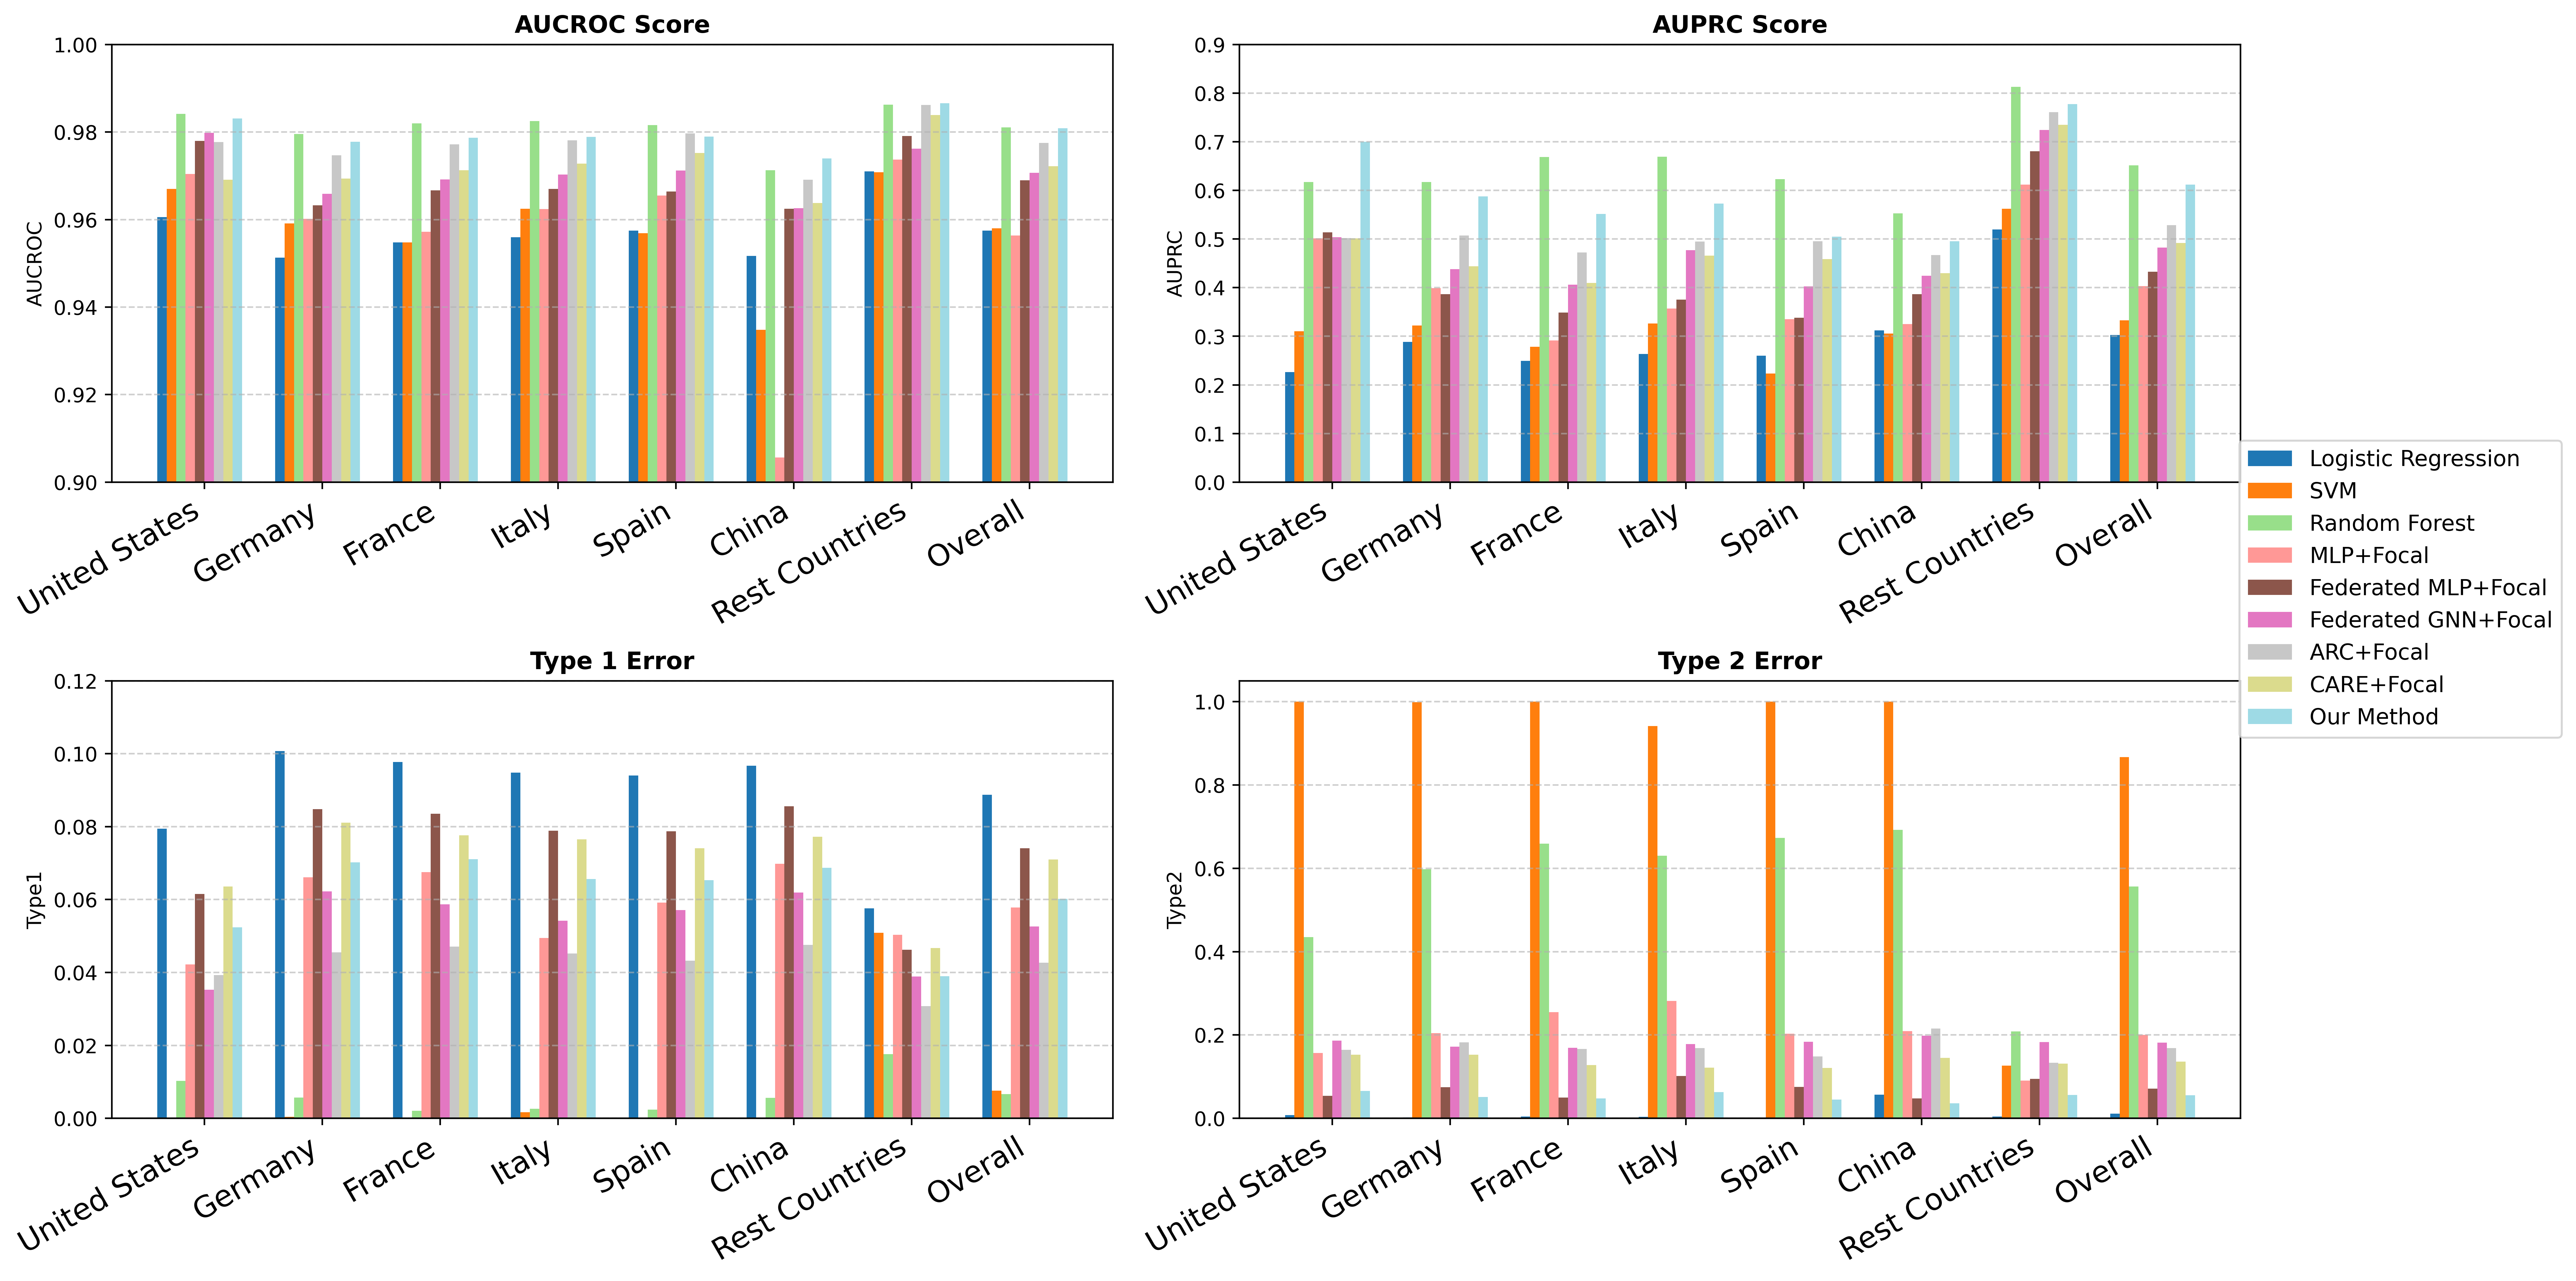
\includegraphics[width=\linewidth]{Detection_model_results/grouped_barcharts_with_legend.png}
    \caption{Comparison with traditional machine learning methods and deep learning approaches. All baseline methods excepted two federated methods are trained on every sub-dataset (i.e., each country) separately.}
    \label{fig:detection_model_results}
\end{figure}


% \begin{figure}[htbp]
%     \centering
%     \centering
%     \includegraphics[width=\linewidth]{Detection_model_results/grouped_barcharts_separate_vs_together.png}
%     \caption{Comparison of country-specific models trained independently with a unified model trained on the aggregated data from all countries.}
%     \label{fig:detection_model_separete_vs_together}
% \end{figure}
 
To evaluate the effectiveness of our proposed method, we compare it against three traditional machine learning algorithms, (i.e., Logistic Regression, Support Vector Machine (SVM), and Random Forest), three deep learning baselines (i.e., a three-layer MLP with Focal Loss, Federated three-layer MLP with Focal Loss and Federated Graph Convolutional Network (GCN) with Focal Loss), and two recent and advanced anomaly detection methods published in top AI Conferences, i.e., CARE~\parencite{zheng2025cluster}, ARC~\parencite{liu2024arc}. Notice that both federated MLP and federated GNN are trained using a federated averaging protocol while ARC is a generalist graph anomaly detection model trained on all sub-datasets. The rest baseline models are trained independently on each sub-dataset (i.e., each country). Figure \ref{fig:detection_model_results} reports the performance of our method relative to these baselines. 

To assess the benefits of federated learning, we compare the standard MLP with the Federated MLP. As shown in Figure \ref{fig:detection_model_results}, the Federated MLP with focal loss achieves higher AUCROC and AUPRC, while also reducing both Type I and Type II errors. We attribute these performance gains to the shared global model parameters maintained under the federated paradigm. By aggregating model updates rather than raw data, federated learning enables the model to capture cross-country behavioral patterns that would be inaccessible in isolated training. This promotes better generalization, reduces overfitting to local data, and allows each client model to benefit from the implicit knowledge of all others without compromising data privacy. In effect, the federated setting provides the model with a richer representation space, boosting predictive stability and robustness across markets.

To understand the value of incorporating structural information from graph data, we further compare Federated GCN with Federated MLP. The results show that Federated GCN achieves higher AUPRC, lower Type I error, and competitive AUCROC, while incurring only a modest increase in Type II error. The performance advantage of Federated GCN stems from its ability to leverage relational structures that encode how accounts interact with one another. These graph-based dependencies capture behavioral patterns that are difficult to learn from tabular features alone. By integrating both local node attributes and cross-account connectivity, Federated GCN can more effectively distinguish normal account behavior from suspicious activities. This structural signal proves pivotal in further boosting detection accuracy.

Two advanced graph anomaly detection methods (i.e., CARE, ARC) achieves better performance than Federated GNN with respect to AUPRC score and lower Type II error due to their special design for identifying the anomalies against the normal nodes, such as maximizing the difference of representations between the anomalies and normal nodes. Overall, our method achieves stronger performance than most competing approaches in terms of AUCROC and AUPRC. Although Random Forest achieves a higher AUPRC than our model, it does so at the expense of substantially higher Type II error (54.5\%), compared with only 5.53\% for our method. This trade-off reflects a model that favors positive predictions but sacrifices recall on the negative class, making it less suitable for money-laundering detection.




\subsubsection{Transferability of Detection Module}

\begin{table}[t]
    \centering
    \caption{Cross-market generalization under leave-one-country-out evaluation}
    \resizebox{\textwidth}{!}{
    \begin{tabular}{l|cccc|cccc}
        \hline
        % \multicolumn{9}{c}{\textbf{All Countries and Leave Germany Out}} \\
        % \hline
        \multirow{2}{*}{\textbf{Market}} 
        & \multicolumn{4}{c|}{\textbf{All Countries}} 
        & \multicolumn{4}{c}{\textbf{Leave Germany out}} \\
        \cline{2-9}
         & AUCROC & AUPRC & Type I & Type II
         & AUCROC & AUPRC & Type I & Type II \\
        \hline
        United States  & 0.9830 & 0.7135 & 0.0513 & 0.0534 & 0.9844 & 0.7257 & 0.0483 & 0.0575 \\
        Germany        & 0.9791 & 0.6047 & 0.0720 & 0.0421 & 0.9792 & 0.5970 & 0.0682 & 0.0512 \\
        France         & 0.9792 & 0.5638 & 0.0704 & 0.0387 & 0.9801 & 0.5674 & 0.0676 & 0.0464 \\
        Italy          & 0.9784 & 0.5678 & 0.0670 & 0.0571 & 0.9792 & 0.5724 & 0.0641 & 0.0645 \\
        Spain          & 0.9809 & 0.5246 & 0.0657 & 0.0334 & 0.9814 & 0.5222 & 0.0629 & 0.0373 \\
        China          & 0.9759 & 0.5131 & 0.0713 & 0.0325 & 0.9755 & 0.5096 & 0.0656 & 0.0423 \\
        Rest Countries & 0.9865 & 0.7791 & 0.0416 & 0.0415 & 0.9864 & 0.7735 & 0.0398 & 0.0558 \\
        \hline
        Overall        & 0.9804 & 0.6095 & 0.0628 &\textbf{0.0427} & 0.9809 & 0.6097 & 0.0595 & 0.0507 \\
        \hline\hline

        % \multicolumn{9}{c}{\textbf{Leave United States Out and Leave China Out}} \\
        % \hline
        \multirow{2}{*}{\textbf{Market}} 
        & \multicolumn{4}{c|}{\textbf{Leave United States out}} 
        & \multicolumn{4}{c}{\textbf{Leave China out}} \\
        \cline{2-9}
         & AUCROC & AUPRC & Type I & Type II
         & AUCROC & AUPRC & Type I & Type II \\
        \hline
        United States  & 0.9787 & 0.6523 & 0.0498 & 0.0927 & 0.9821 & 0.7139 & 0.0485 & 0.0796 \\
        Germany        & 0.9799 & 0.6093 & 0.0660 & 0.0398 & 0.9781 & 0.5869 & 0.0671 & 0.0603 \\
        France         & 0.9808 & 0.5976 & 0.0655 & 0.0588 & 0.9781 & 0.5702 & 0.0672 & 0.0604 \\
        Italy          & 0.9819 & 0.6199 & 0.0599 & 0.0626 & 0.9783 & 0.5809 & 0.0635 & 0.0645 \\
        Spain          & 0.9818 & 0.5529 & 0.0599 & 0.0452 & 0.9805 & 0.5230 & 0.0625 & 0.0373 \\
        China          & 0.9764 & 0.5266 & 0.0643 & 0.0488 & 0.9733 & 0.4951 & 0.0635 & 0.0520 \\
        Rest Countries & 0.9873 & 0.8001 & 0.0402 & 0.0399 & 0.9866 & 0.7829 & 0.0389 & 0.0590 \\
        \hline
        Overall        & \textbf{0.9810} & \textbf{0.6227} & \textbf{0.0579} & 0.0554 & 0.9796 & 0.6075 & 0.0588 & 0.0590 \\
        \hline
    \end{tabular}}
    \label{tab:leave_one_country_out}
\end{table}

Although the proposed system demonstrates strong in-sample performance, a central question is whether the learned financial intelligence generalizes to markets unseen during training. To examine this, we conduct a leave-one-country-out evaluation, in which the model is trained on all countries except one and then tested on the excluded market, mimicking deployment in a new or emerging jurisdiction. As shown in Table~\ref{tab:leave_one_country_out}, overall detection performance remains remarkably stable across all hold-out scenarios. Relative to the full-data benchmark (overall AUCROC = 0.9804, AUPRC = 0.6095), excluding Germany has virtually no impact on global performance (AUCROC = 0.9809), while excluding the United States slightly improves overall AUPRC to 0.6227, indicating that the learned representations are not overly dependent on any single market. At the market (country) level, performance degradation on the held-out country is modest and economically interpretable. When the United States is excluded from training, the U.S. subgraph exhibits an increase in Type II error from 5.3\% to 9.3\%, reflecting the absence of high-volume, highly connected transaction patterns during training. At the same time, detection performance in other countries improves, with AUPRC increasing to 0.6093 in Germany and 0.6199 in Italy. This pattern is consistent with the disproportionate scale of the U.S. market (approximately 855k transactions) relative to other countries (each below 250k), suggesting that training without the dominant market encourages the model to learn more balanced and transferable transaction structures. A similar but weaker effect is observed when China is held out. The China subgraph experiences only a moderate increase in Type II error (from 3.3\% to 5.2\%), while overall performance remains close to the baseline (AUCROC = 0.9796), indicating robust generalization even to structurally distinct financial ecosystems. Across all settings, detection performance in smaller and less-connected markets (“Rest Countries”) remains consistently high, with AUCROC exceeding 0.986. 

Overall, these results provide strong evidence that the proposed system captures structural laundering patterns that generalize across countries rather than country-specific transaction idiosyncrasies. While excluding a dominant financial hub predictably reduces performance in that specific market, global detection capability remains stable and, in some cases, improves elsewhere. This highlights the system’s potential to support scalable cross-border deployment and to bootstrap effective anti-money-laundering detection in new or data-scarce markets without extensive local historical data.


\begin{table}[t]
    \centering
    \caption{Communication frequency vs. performance in federated learning}
    \label{tab:communication_fed}
    \resizebox{\textwidth}{!}{
    \begin{tabular}{l|cccc|cccc}
        \hline
        \multirow{2}{*}{\textbf{Market}} 
        & \multicolumn{4}{c|}{\textbf{frequency=1 }} 
        & \multicolumn{4}{c}{\textbf{frequency=1/2 }} \\
        \cline{2-9}
         & AUCROC & AUPRC & Type I & Type II
         & AUCROC & AUPRC & Type I & Type II \\
        \hline
        United States  & 0.9790 & 0.6659 & 0.0230 & 0.1935 & 0.9795 & 0.6812 & 0.0392 & 0.1048 \\
        Germany        & 0.9766 & 0.5584 & 0.0296 & 0.2059 & 0.9787 & 0.5884 & 0.0524 & 0.1081 \\
        France         & 0.9773 & 0.5301 & 0.0298 & 0.1734 & 0.9785 & 0.5391 & 0.0545 & 0.0805 \\
        Italy          & 0.9787 & 0.5691 & 0.0253 & 0.2284 & 0.9790 & 0.5684 & 0.0484 & 0.1105 \\
        Spain          & 0.9784 & 0.5073 & 0.0254 & 0.2083 & 0.9794 & 0.5036 & 0.0504 & 0.0884 \\
        China          & 0.9726 & 0.4735 & 0.0304 & 0.2520 & 0.9727 & 0.4968 & 0.0526 & 0.1122 \\
        Rest Countries & 0.9858 & 0.7883 & 0.0229 & 0.1866 & 0.9864 & 0.7765 & 0.0328 & 0.0909 \\
        \hline
        Overall        & 0.9783 & 0.5847 & 0.0266 & 0.2069 & 0.9792 & 0.5934 & 0.0472 & 0.0993 \\
        \hline
    \end{tabular}}

    \resizebox{\textwidth}{!}{
    \begin{tabular}{l|cccc|cccc}
        \hline
        \multirow{2}{*}{\textbf{Market}} 
        & \multicolumn{4}{c|}{\textbf{frequency=1/4}} 
        & \multicolumn{4}{c}{\textbf{frequency=1/8}} \\
        \cline{2-9}
         & AUCROC & AUPRC & Type I & Type II
         & AUCROC & AUPRC & Type I & Type II \\
        \hline
        United States  & 0.9830 & 0.7135 & 0.0513 & 0.0534 & 0.9824 & 0.7195 & 0.0494 & 0.0635 \\
        Germany        & 0.9791 & 0.6047 & 0.0720 & 0.0421 & 0.9792 & 0.5944 & 0.0672 & 0.0501 \\
        France         & 0.9792 & 0.5638 & 0.0704 & 0.0387 & 0.9807 & 0.5849 & 0.0670 & 0.0480 \\
        Italy          & 0.9784 & 0.5678 & 0.0670 & 0.0571 & 0.9792 & 0.5899 & 0.0635 & 0.0700 \\
        Spain          & 0.9809 & 0.5246 & 0.0657 & 0.0334 & 0.9809 & 0.5277 & 0.0625 & 0.0452 \\
        China          & 0.9759 & 0.5131 & 0.0713 & 0.0325 & 0.9757 & 0.5151 & 0.0657 & 0.0488 \\
        Rest Countries & 0.9865 & 0.7791 & 0.0416 & 0.0415 & 0.9873 & 0.7947 & 0.0394 & 0.0526 \\
        \hline
        Overall        & 0.9804 & 0.6095 & 0.0628 & 0.0427 & \textbf{0.9808} & \textbf{0.6180} & 0.0593 & 0.0540 \\
        \hline
    \end{tabular}}
\end{table}

\subsubsection{Communication Frequency of Detection Module}
To quantify the efficiency–accuracy trade-off in federated learning, we vary the communication frequency while holding the total training budget fixed. We fixed the training epochs to 4000 and vary the communication frequency from 1 to 1/2, 1/4, and 1/8 (communicate once every 8 epochs). Notice that the lower communication frequency mean the lower local updates before aggregation. Table~\ref{tab:communication_fed} reports a clear and economically meaningful pattern. When communication occurs every epoch (frequency=1), the system exhibits severe underperformance, with an overall AUPRC of 0.5847 and a Type II error rate of 20.7\%, indicating that overly frequent synchronization prevents institutions from adequately learning localized transaction structures. Halving the communication interval (frequency=1/2) improves AUPRC by nearly 0.9\% (from 0.5847 to 0.5934) and cuts the Type II error rate by more than half (from 20.7\% to 9.9\%), suggesting substantial gains from allowing richer local updates before aggregation. Performance improves when we further halve the communication frequencies. At frequency=1/4, the system achieves an overall AUPRC of 0.6095 with a 2.5\% improvement relative to frequency=1, while greatly reducing the Type II error from 20.69\% to 4.3\%. This improvement is consistent across all major countries/markets for example, in the United States subgraph, the missed-detection rate drops from 19.4\% at frequency=1 to 5.3\% at frequency=1/4, while AUPRC increases from 0.666 to 0.714. Importantly, these gains are obtained with a fourfold reduction in communication rounds, highlighting a strong efficiency payoff. Moving to an even lower communication regime (frequency=1/8) yields diminishing but still positive returns. While overall AUPRC increases slightly to 0.6180, Type II error rises modestly to 5.4\%, indicating a trade-off between recall and communication sparsity. This pattern suggests that excessively infrequent synchronization can introduce model drift across institutions, particularly in heterogeneous markets such as China and Italy. Nevertheless, even at frequency=1/8, performance remains substantially superior to high-frequency communication, with a 74\% reduction in missed detections relative to frequency=1.

These results demonstrate that federated efficiency in cross-border anti-money-laundering systems is non-monotonic in communication frequency. Moderate synchronization intervals dominate both extremes by simultaneously improving detection accuracy and reducing communication costs. This implies that regulators and financial institutions can achieve higher detection effectiveness while substantially lowering coordination and compliance overhead by avoiding overly frequent model aggregation. The findings provide practical guidance for designing scalable, privacy-preserving financial intelligence systems in globally distributed settings.


\subsubsection{Granularity of super-node sharing}
\label{supernode_high_order_results}1
In this section, we aim to investigate the impact of varying the granularity of supernode feature sharing by comparing two aggregation strategies: using only the mean of connected node features (first-order statistical moment) versus using both the mean and variance (first-order and second-order statistical moment). Table~\ref{tab:supernode_aggregation} shows that the differences in overall performance between the two approaches are minimal. While the mean + variance aggregation slightly reduces Type II errors in some markets (e.g., Germany, Spain, China), it also increases Type I errors in others (e.g., United States, France). Across all markets, AUCROC and AUPRC remain largely stable, indicating that incorporating higher-order moments beyond the first has diminishing returns. These results suggest that capturing the first moment (mean) of supernode features is sufficient for effective detection, and additional statistics such as variance provide only marginal benefits relative to the added complexity of computation and communication in a cross-bank setting. Therefore, a simple mean-based aggregation offers a favorable trade-off between performance and efficiency for supernode sharing in heterogeneous financial networks.
\begin{table}[htbp]
\centering
\caption{Comparison of supernode feature aggregation strategies: Mean aggregation vs. Mean + Variance aggregation. Performance is reported for each market in terms of AUC, Average Precision (AP), Type I error, and Type II error.}
\resizebox{\textwidth}{!}{
\begin{tabular}{lcccc|cccc}
\hline
\multirow{2}{*}{\textbf{Market}} & \multicolumn{4}{c|}{\textbf{Mean Aggregation}} & \multicolumn{4}{c}{\textbf{Mean + Variance Aggregation}} \\
\cline{2-9}
 & \textbf{AUCROC} & \textbf{AUPRC} & \textbf{Type I} & \textbf{Type II} & \textbf{AUCROC} & \textbf{AUPRC} & \textbf{Type I} & \textbf{Type II} \\
\hline
United States & 0.9824 & 0.7195 & 0.0494 & 0.0635 & 0.9825 & 0.6951 & 0.0540 & 0.0625 \\
Germany       & 0.9792 & 0.5944 & 0.0672 & 0.0501 & 0.9789 & 0.5960 & 0.0719 & 0.0375 \\
France        & 0.9807 & 0.5849 & 0.0670 & 0.0480 & 0.9802 & 0.5850 & 0.0717 & 0.0433 \\
Italy         & 0.9792 & 0.5899 & 0.0635 & 0.0700 & 0.9788 & 0.5921 & 0.0658 & 0.0497 \\
Spain         & 0.9809 & 0.5277 & 0.0625 & 0.0452 & 0.9807 & 0.5372 & 0.0669 & 0.0334 \\
China         & 0.9757 & 0.5151 & 0.0657 & 0.0488 & 0.9751 & 0.5064 & 0.0697 & 0.0325 \\
Rest Countries & 0.9873 & 0.7947 & 0.0394 & 0.0526 & 0.9861 & 0.8003 & 0.0412 & 0.0351 \\
\hline
\textbf{Overall} & \textbf{0.9808} & \textbf{0.6180} & \textbf{0.0593} & 0.0540 & 0.9803 & 0.6160 & 0.0630 & \textbf{0.0420} \\
\hline
\end{tabular}}
\label{tab:supernode_aggregation}
\end{table}


\begin{table}[h!]
\centering
\caption{Statistics of transaction by country}
\resizebox{0.9\textwidth}{!}{
\begin{tabular}{lcccc}
\hline
\textbf{Country} & \textbf{\#Accounts} & \textbf{\#Total Transactions} & \textbf{\#Illicit Transactions} & \textbf{Ratio of Illicity}\\
\hline
United States   & 396,370 & 4,175,722   & 3,489     & 0.084\%\\
Germany         & 197,543 & 1,599,846   & 1,542     & 0.096\%\\
France          & 168,372 & 1,284,859   & 1,145     & 0.089\%\\
Italy           & 149,425 & 1,082,159   & 977       & 0.090\%\\
Spain           & 137,726 & 989,019     & 911       & 0.092\%\\
China           & 130,099 & 973,821     & 1,050     & 0.011\%\\
Rest Countries  & 278,480 & 1,700,615   & 1,284     & 0.076\%\\
\hline
Overall         & 208,288 & 1,686,577   & 1,485     & 0.077\%\\
\hline
\end{tabular}}
\label{tab:country_graph_stats_full}
\end{table}

\subsubsection{Scalability to Enterprise-Level Transaction Volumes}
\label{scalability_analysis}
% In this section, we demonstrate the scalability of our detection module. We summarize the transaction networks across different countries in Table~\ref{tab:country_graph_stats_full} for the subset with 5 million transaction records. 
We evaluate the detection module on the full IBM AML dataset comprising over 5 million transactions (Table \ref{tab:country_graph_stats_full}). This setting presents substantially greater challenges than the primary experiments: the illicit transaction ratio drops to approximately 0.08\%—nearly five times more imbalanced than the 1.4 million transaction subset—and the labeled training data is limited to 20\% of transactions, reflecting realistic constraints on investigator capacity for manual labeling.

Table~\ref{scalability_analysis} reports the results. The baseline GNN with focal loss exhibits severe majority-class bias, achieving low Type I error (0.33\%) but unacceptably high Type II error (62.96\%), indicating that the model learns to classify nearly all transactions as legitimate. Our method, combining federated graph learning with structure-preserving downsampling (20:1 ratio), substantially improves detection sensitivity: Type II error decreases from 62.96\% to 23.13\%—a 63\% reduction in missed illicit transactions. This improvement comes at the cost of moderately higher Type I error (6.79\%), reflecting the fundamental precision-recall trade-off under extreme imbalance.


Several observations merit discussion. First, the performance gap between the 1.4M and 5M transaction settings highlights the compounding difficulty of extreme class imbalance: at 0.08\% positive rate, even focal loss struggles to prevent majority-class dominance. Second, AUPRC scores (0.33 overall) are lower than in the smaller dataset, consistent with the information-theoretic limits of learning from very few positive examples per training batch. Third, cross-country heterogeneity persists, with "Rest Countries" showing the weakest performance (Type II = 29.02\%), potentially reflecting greater distributional shift in smaller, less-regulated markets.

 
These results suggest two directions for improvement that we leave to future work: (1) increasing the proportion of labeled training data, which is constrained by investigator capacity in practice, and (2) developing curriculum learning strategies that progressively increase task difficulty as the model learns basic laundering patterns. Despite these limitations, the substantial reduction in Type II error demonstrates that our framework provides meaningful detection improvements even at enterprise scale, where baseline methods effectively fail.

\begin{table*}[ht!]
\centering
\caption{Performance Comparison Between Our Method and the Baseline Method (GNN with Focal Loss)}
\small
\resizebox{0.95\textwidth}{!}{
\begin{tabular}{l|cccc|cccc}
\hline
\multirow{2}{*}{\textbf{Markets}} 
& \multicolumn{4}{c|}{\textbf{Our Method}} 
& \multicolumn{4}{c}{\textbf{GNN + Focal Loss}} \\
\cline{2-9}
& AUCROC & AUPRC & Type I & Type II 
& AUCROC & AUPRC & Type I & Type II \\
\hline
United States & 0.9667 & 0.4407 & 0.0554 & 0.2164 & 0.9693 & 0.3867 & 0.0036 & 0.5550 \\
Germany       & 0.9619 & 0.3941 & 0.0688 & 0.2156 & 0.9684 & 0.3728 & 0.0034 & 0.5932 \\
France        & 0.9608 & 0.3438 & 0.0694 & 0.2074 & 0.9664 & 0.3593 & 0.0033 & 0.5841 \\
Italy         & 0.9510 & 0.2937 & 0.0776 & 0.2570 & 0.9635 & 0.2655 & 0.0027 & 0.7110 \\
Spain         & 0.9556 & 0.2887 & 0.0804 & 0.2373 & 0.9644 & 0.3565 & 0.0028 & 0.6296 \\
China         & 0.9657 & 0.3129 & 0.0649 & 0.1952 & 0.9672 & 0.3285 & 0.0043 & 0.6155 \\
Rest Countries     & 0.9523 & 0.2231 & 0.0586 & 0.2902 & 0.9549 & 0.1842 & 0.0030 & 0.7186 \\
\hline
Overall             & 0.9591 & \textbf{0.3281} & 0.0679 & \textbf{0.2313} 
                    & \textbf{0.9649} & 0.3219 & \textbf{0.0033} & 0.6296 \\
\hline
\end{tabular}
}
\label{scalability_analysis}
\end{table*}




\subsection{Empirical Results of Cross-bank PPR}
\subsubsection{Interpretation via Identified Group Patterns}
\label{PPR_interpretation}

\begin{figure}[htbp]
    \centering
    % First row
    \vspace{-3mm}
    \begin{subfigure}{0.5\linewidth}
        \centering
        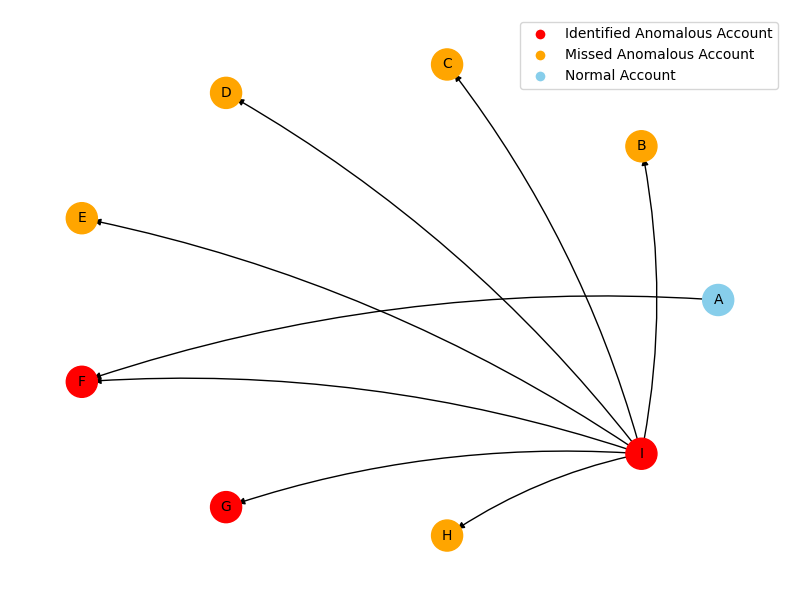
\includegraphics[width=\linewidth]{Interpretability_figure/fan-out.png}
        \caption{Pattern with Fan-out Structure}
    \end{subfigure}%
    \hfill
    \begin{subfigure}{0.5\linewidth}
        \centering
        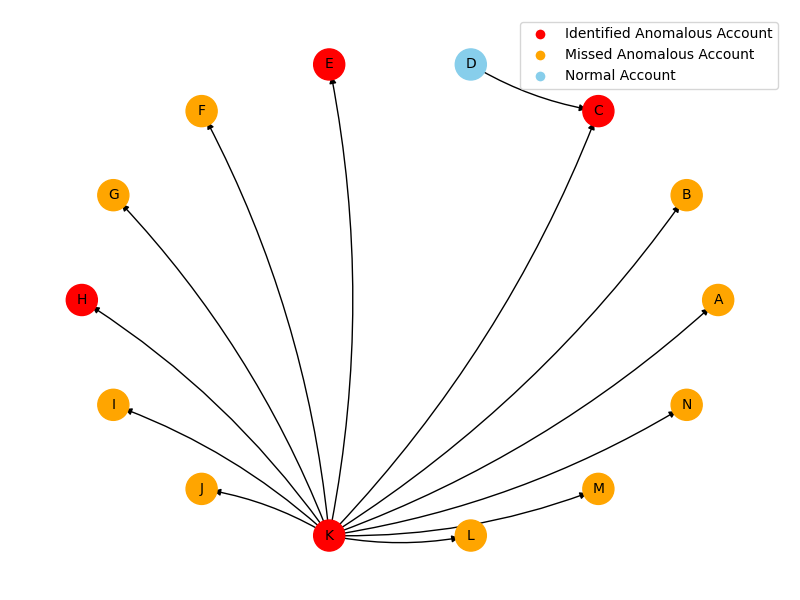
\includegraphics[width=\linewidth]{Interpretability_figure/fan-out_2.png}
        \caption{Pattern with Another Fan-out Structure}
    \end{subfigure}%
    \vspace{0.5em} % small vertical space between rows
    
    % % Second row
    \vspace{-3mm}
    \begin{subfigure}{0.5\linewidth}
        \centering
        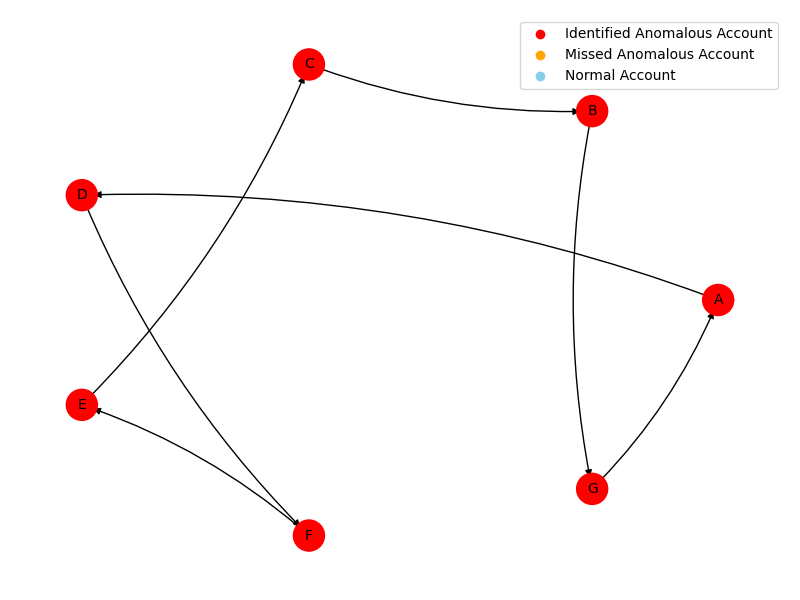
\includegraphics[width=\linewidth]{Interpretability_figure/loop.png}
        \caption{Pattern with Loop Structure}
    \end{subfigure}%
    \hfill
    \begin{subfigure}{0.5\linewidth}
        \centering
        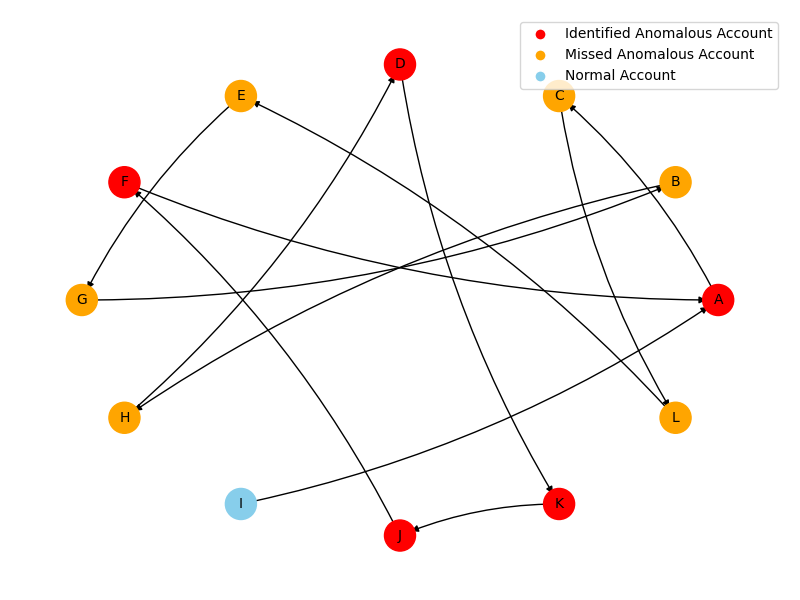
\includegraphics[width=\linewidth]{Interpretability_figure/loop_2.png}
        \caption{Another Pattern with Loop Structure}
    \end{subfigure}
    \vspace{0.5em} % small vertical space between rows
    
    % Third row
    \vspace{-3mm}
    \begin{subfigure}{0.5\linewidth}
        \centering
        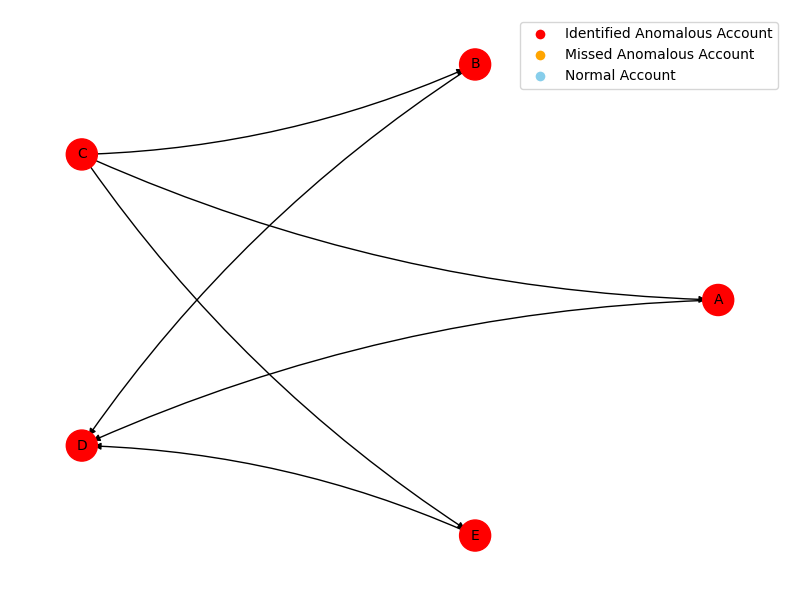
\includegraphics[width=\linewidth]{Interpretability_figure/gather_scatter.png}
        \caption{Pattern with Gather-scatter Structure}
    \end{subfigure}%
    \hfill
    \begin{subfigure}{0.5\linewidth}
        \centering
        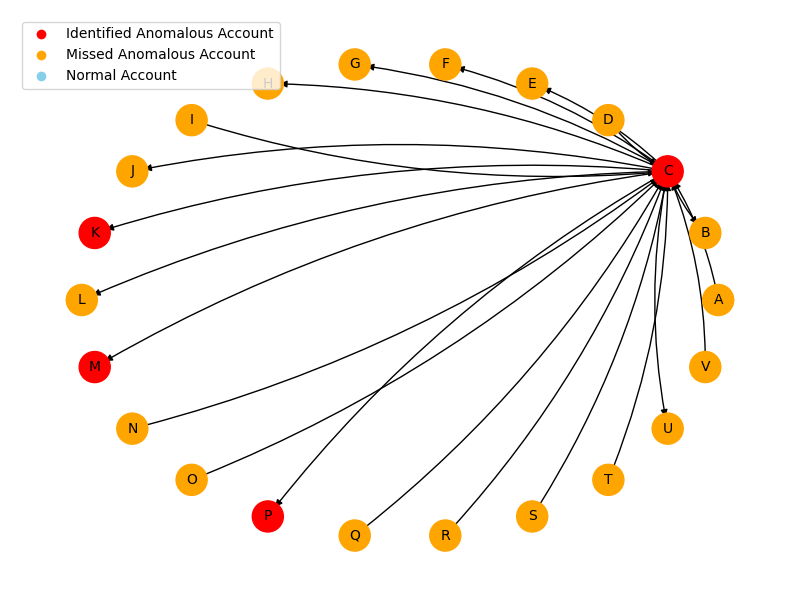
\includegraphics[width=\linewidth]{Interpretability_figure/gather_scatter_fan_out.png}
        \caption{Pattern with Gather and Fan-out Structure}
    \end{subfigure}
    % \vspace{-3mm}
    \caption{Identified Group Money-Laundering Patterns}
    \label{fig:money_laundering_demo}
\end{figure}


We examine the interpretability of group money-laundering patterns identified by the cross-bank Personalized PageRank method. Figure~\ref{fig:money_laundering_demo} illustrates representative patterns detected from the merged transaction clusters. We focus on four distinct types of money-laundering patterns: fan-out, loop, gather-scatter, and hybrid structures combining gather and fan-out mechanisms.

Figures~\ref{fig:money_laundering_demo} (a) and (b) depict fan-out structures, in which funds from a single account are distributed to multiple downstream accounts, reflecting the dispersal behavior commonly used to obscure illicit money flows. In Figure~\ref{fig:money_laundering_demo} (a), funds originate from account I and are distributed to accounts B, C, D, E, F, G, and H. Account A is a normal account incorrectly flagged as suspicious, highlighting the need for further expert review to refine labels. Importantly, our method correctly identifies the primary control account I, which orchestrates the laundering activity. Some accounts, such as B, C, D, E and H, are missed, which we attribute to the “bank isolation” issue, where complete group structures are fragmented across institutions, complicating detection. Similarly, in Figure~\ref{fig:money_laundering_demo} (b), our method correctly identifies account K as the principal node managing the funds.

Figures~\ref{fig:money_laundering_demo} (c) and (d) illustrate loop structures, where funds circulate among accounts before returning to the origin, representing more sophisticated laundering strategies. In Figure~\ref{fig:money_laundering_demo} (c), our method successfully identifies the full loop: funds flow from account A to D, then through accounts D–G, before returning to A. In Figure~\ref{fig:money_laundering_demo} (d), laundering begins at account B in China, with funds moving across accounts in Europe and the United States along multiple chains, including $B \rightarrow H \rightarrow D$ (Europe-based chain), $D \rightarrow K \rightarrow J \rightarrow F \rightarrow A$ (United States-based chain) and  $A \rightarrow C \rightarrow L$ (Europe-based chain). Our method captures the U.S.-based chain but misses the cross-border components, illustrating the challenges posed by fragmented international transactions. Despite partial detection, identifying even a segment of the loop provides valuable signals of illicit activity.

Figures~\ref{fig:money_laundering_demo} (e) and (f) demonstrate gather-scatter mechanisms and hybrid structure combining gather-scatter and fan-out mechanisms, where multiple accounts funnel funds into a central account before redistribution. In Figure~\ref{fig:money_laundering_demo} (e), account C distributes funds to accounts A, B, and E, and account D gather all money flows, completing the laundering cycle, which our method successfully detects. In Figure~\ref{fig:money_laundering_demo} (f), a more complex behavior emerges: account C gathers funds from multiple sources and redistributes them to multiple recipients. While only four of the 22 suspicious accounts are identified, account C is correctly flagged as the pivotal node orchestrating the activity.

These results provide a clear interpretation of group money-laundering behaviors by revealing the underlying relational structures within transaction networks. By identifying patterns such as fan-out, loop, gather-scatter, and hybrid mechanisms, the method highlights how funds flow between accounts and pinpoints the pivotal nodes that orchestrate these operations. Even when full laundering cycles are fragmented across banks or countries, the detection of key control accounts and partial transaction chains offers interpretable insights into the mechanisms of illicit activity. This structural perspective allows analysts to understand not only which accounts are suspicious, but also how money moves through the network, supporting more informed decision-making, targeted investigations, and effective regulatory interventions.


\begin{figure}[htbp]
    \centering
    % First row
    \vspace{-3mm}
    \begin{subfigure}{0.5\linewidth}
        \centering
        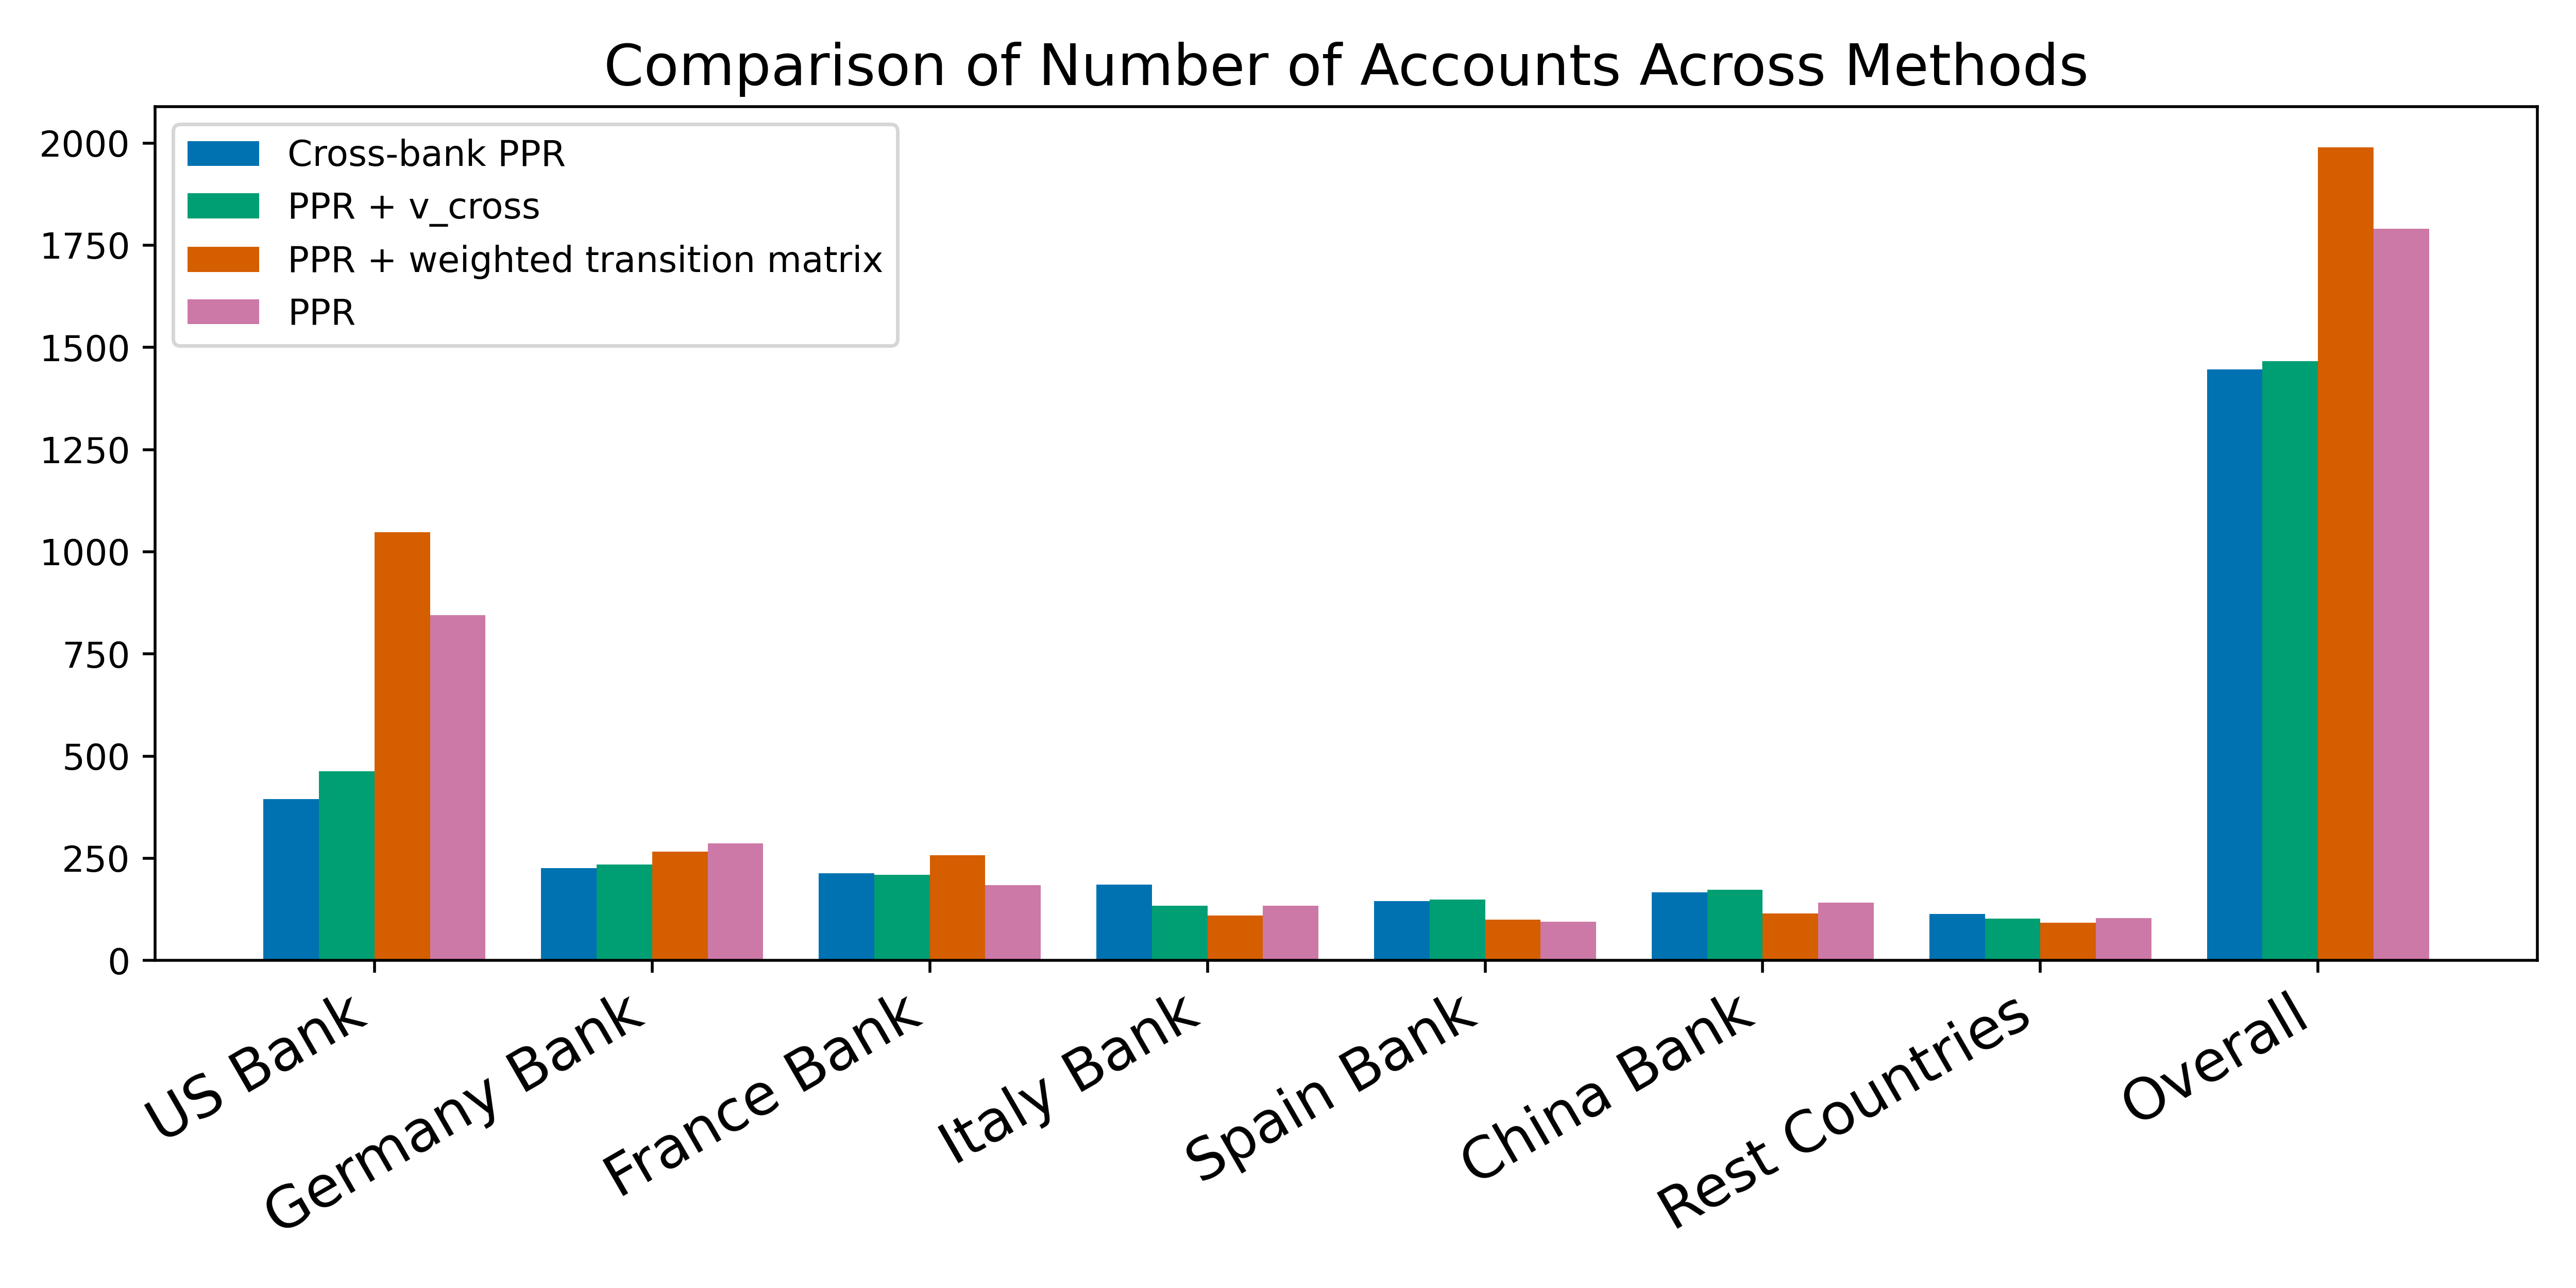
\includegraphics[width=\linewidth]{PPR_results/Account.png}
        \begin{center}
            \caption{Total number of accounts included \\
            across all clusters}
        \end{center}
    \end{subfigure}%
    \hfill
    \begin{subfigure}{0.5\linewidth}
        \centering
        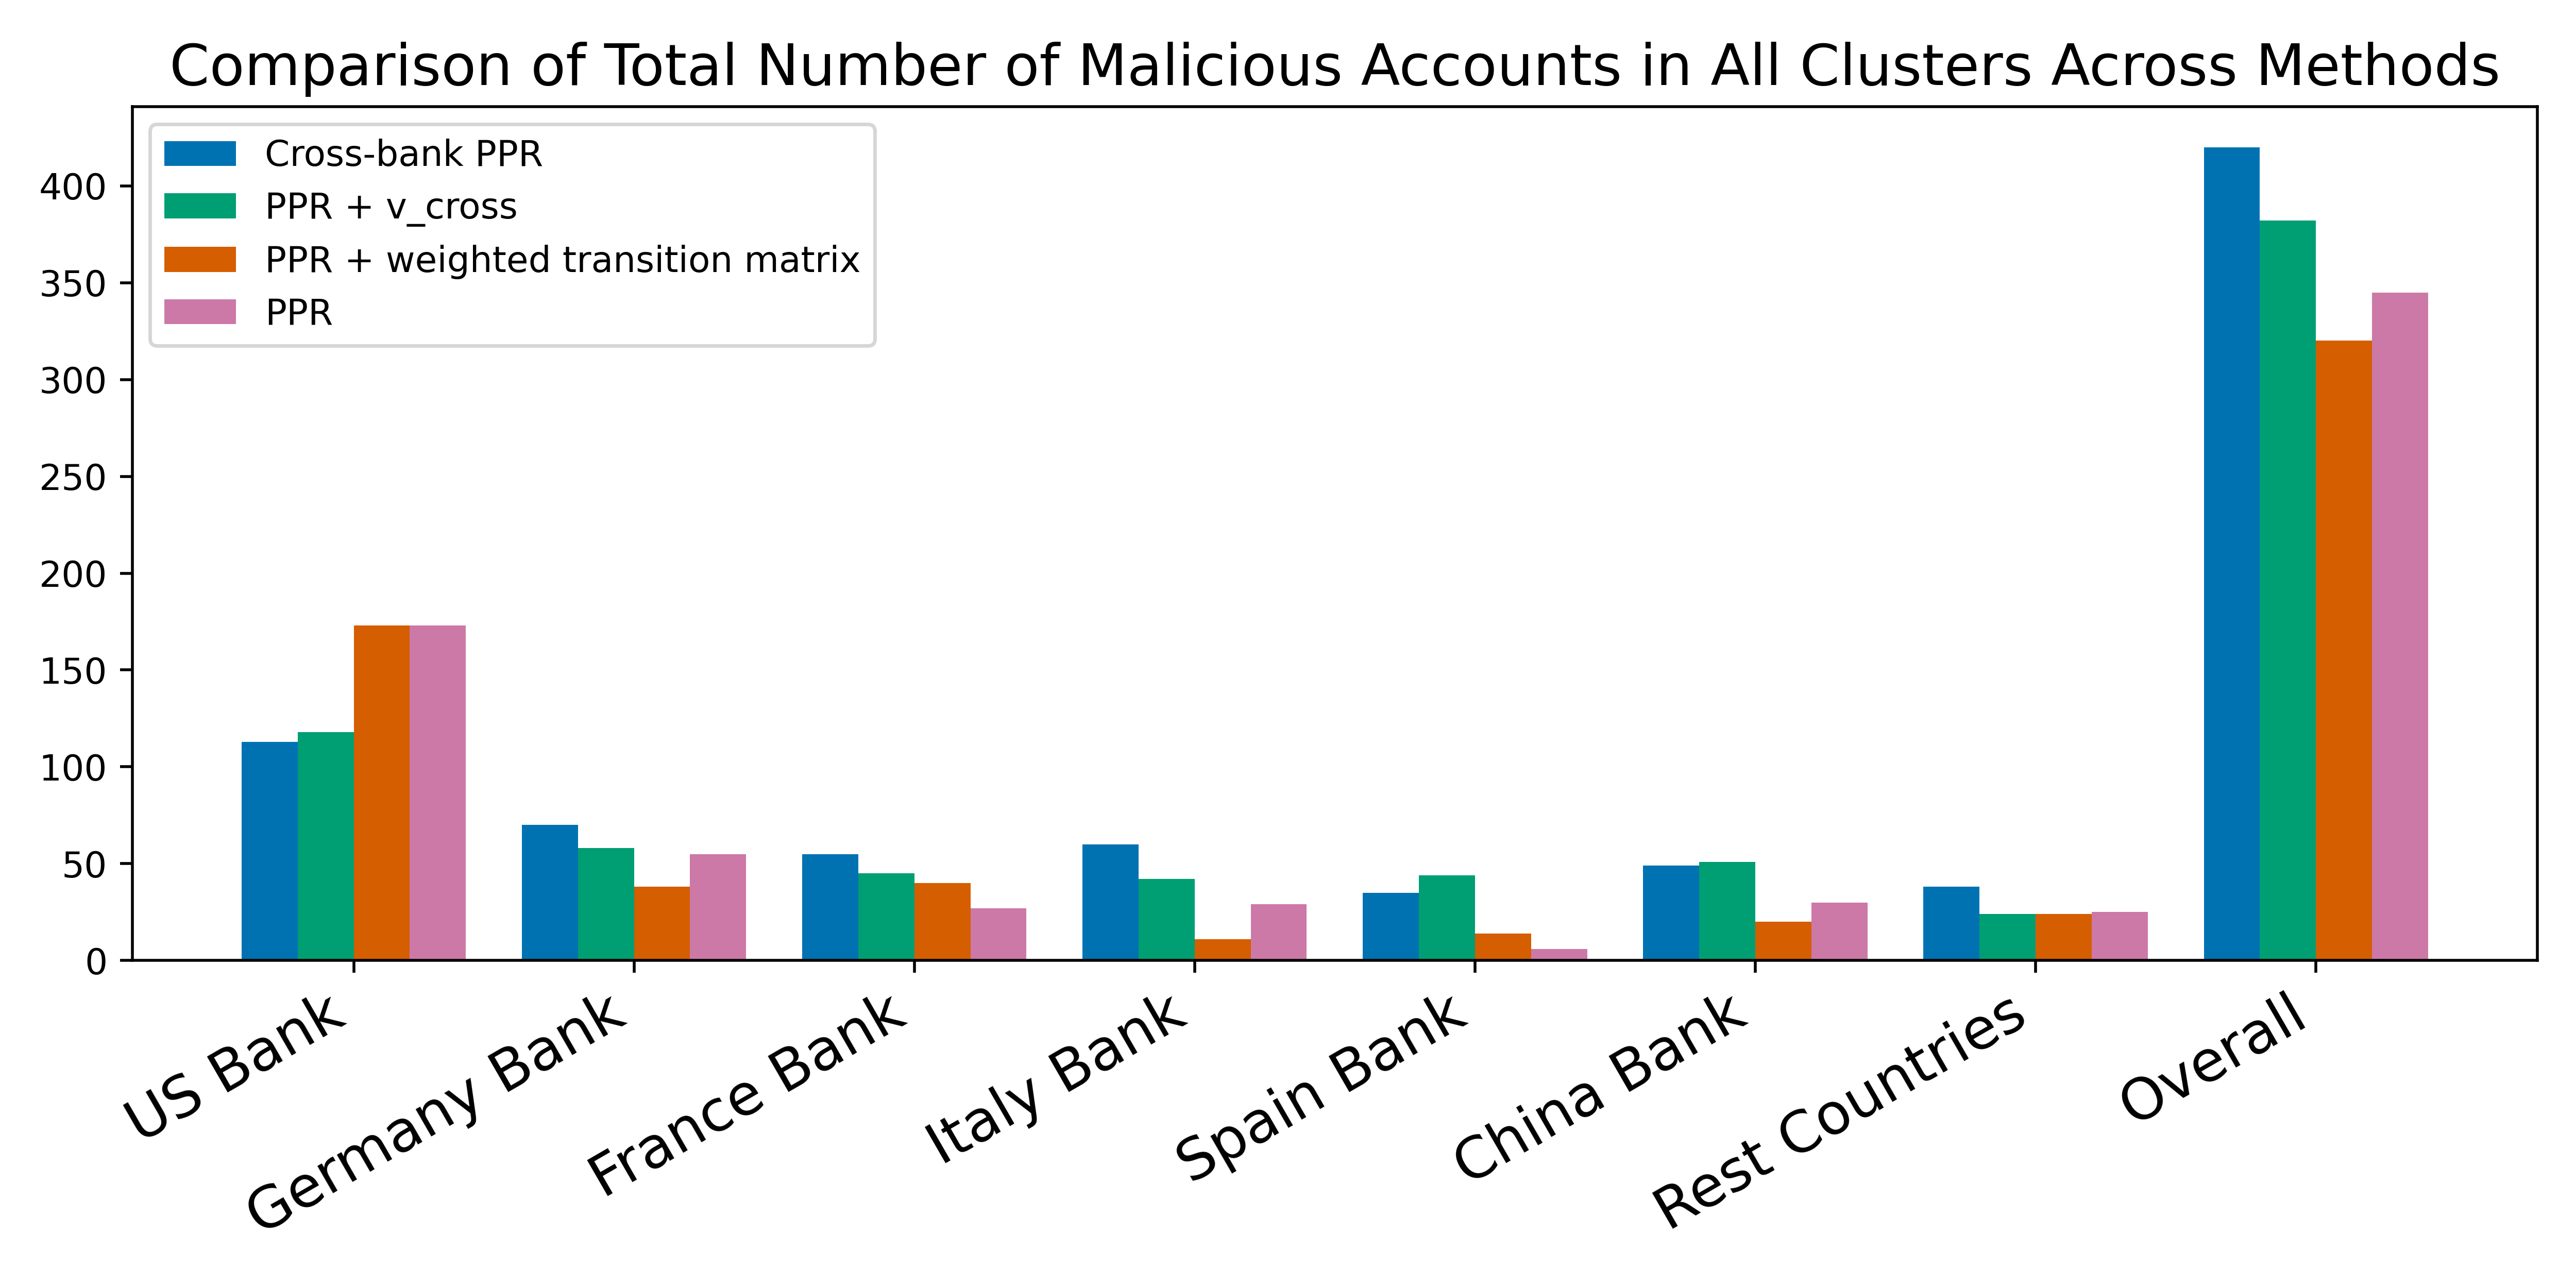
\includegraphics[width=\linewidth]{PPR_results/Anomalies.png}
        \begin{center}
            \caption{Number of malicious accounts  \\
            in all clusters}
        \end{center}
    \end{subfigure}%
    \vspace{0.5em} % small vertical space between rows
    
    % % Second row
    % \vspace{-3mm}
    \begin{subfigure}{0.5\linewidth}
        \centering
        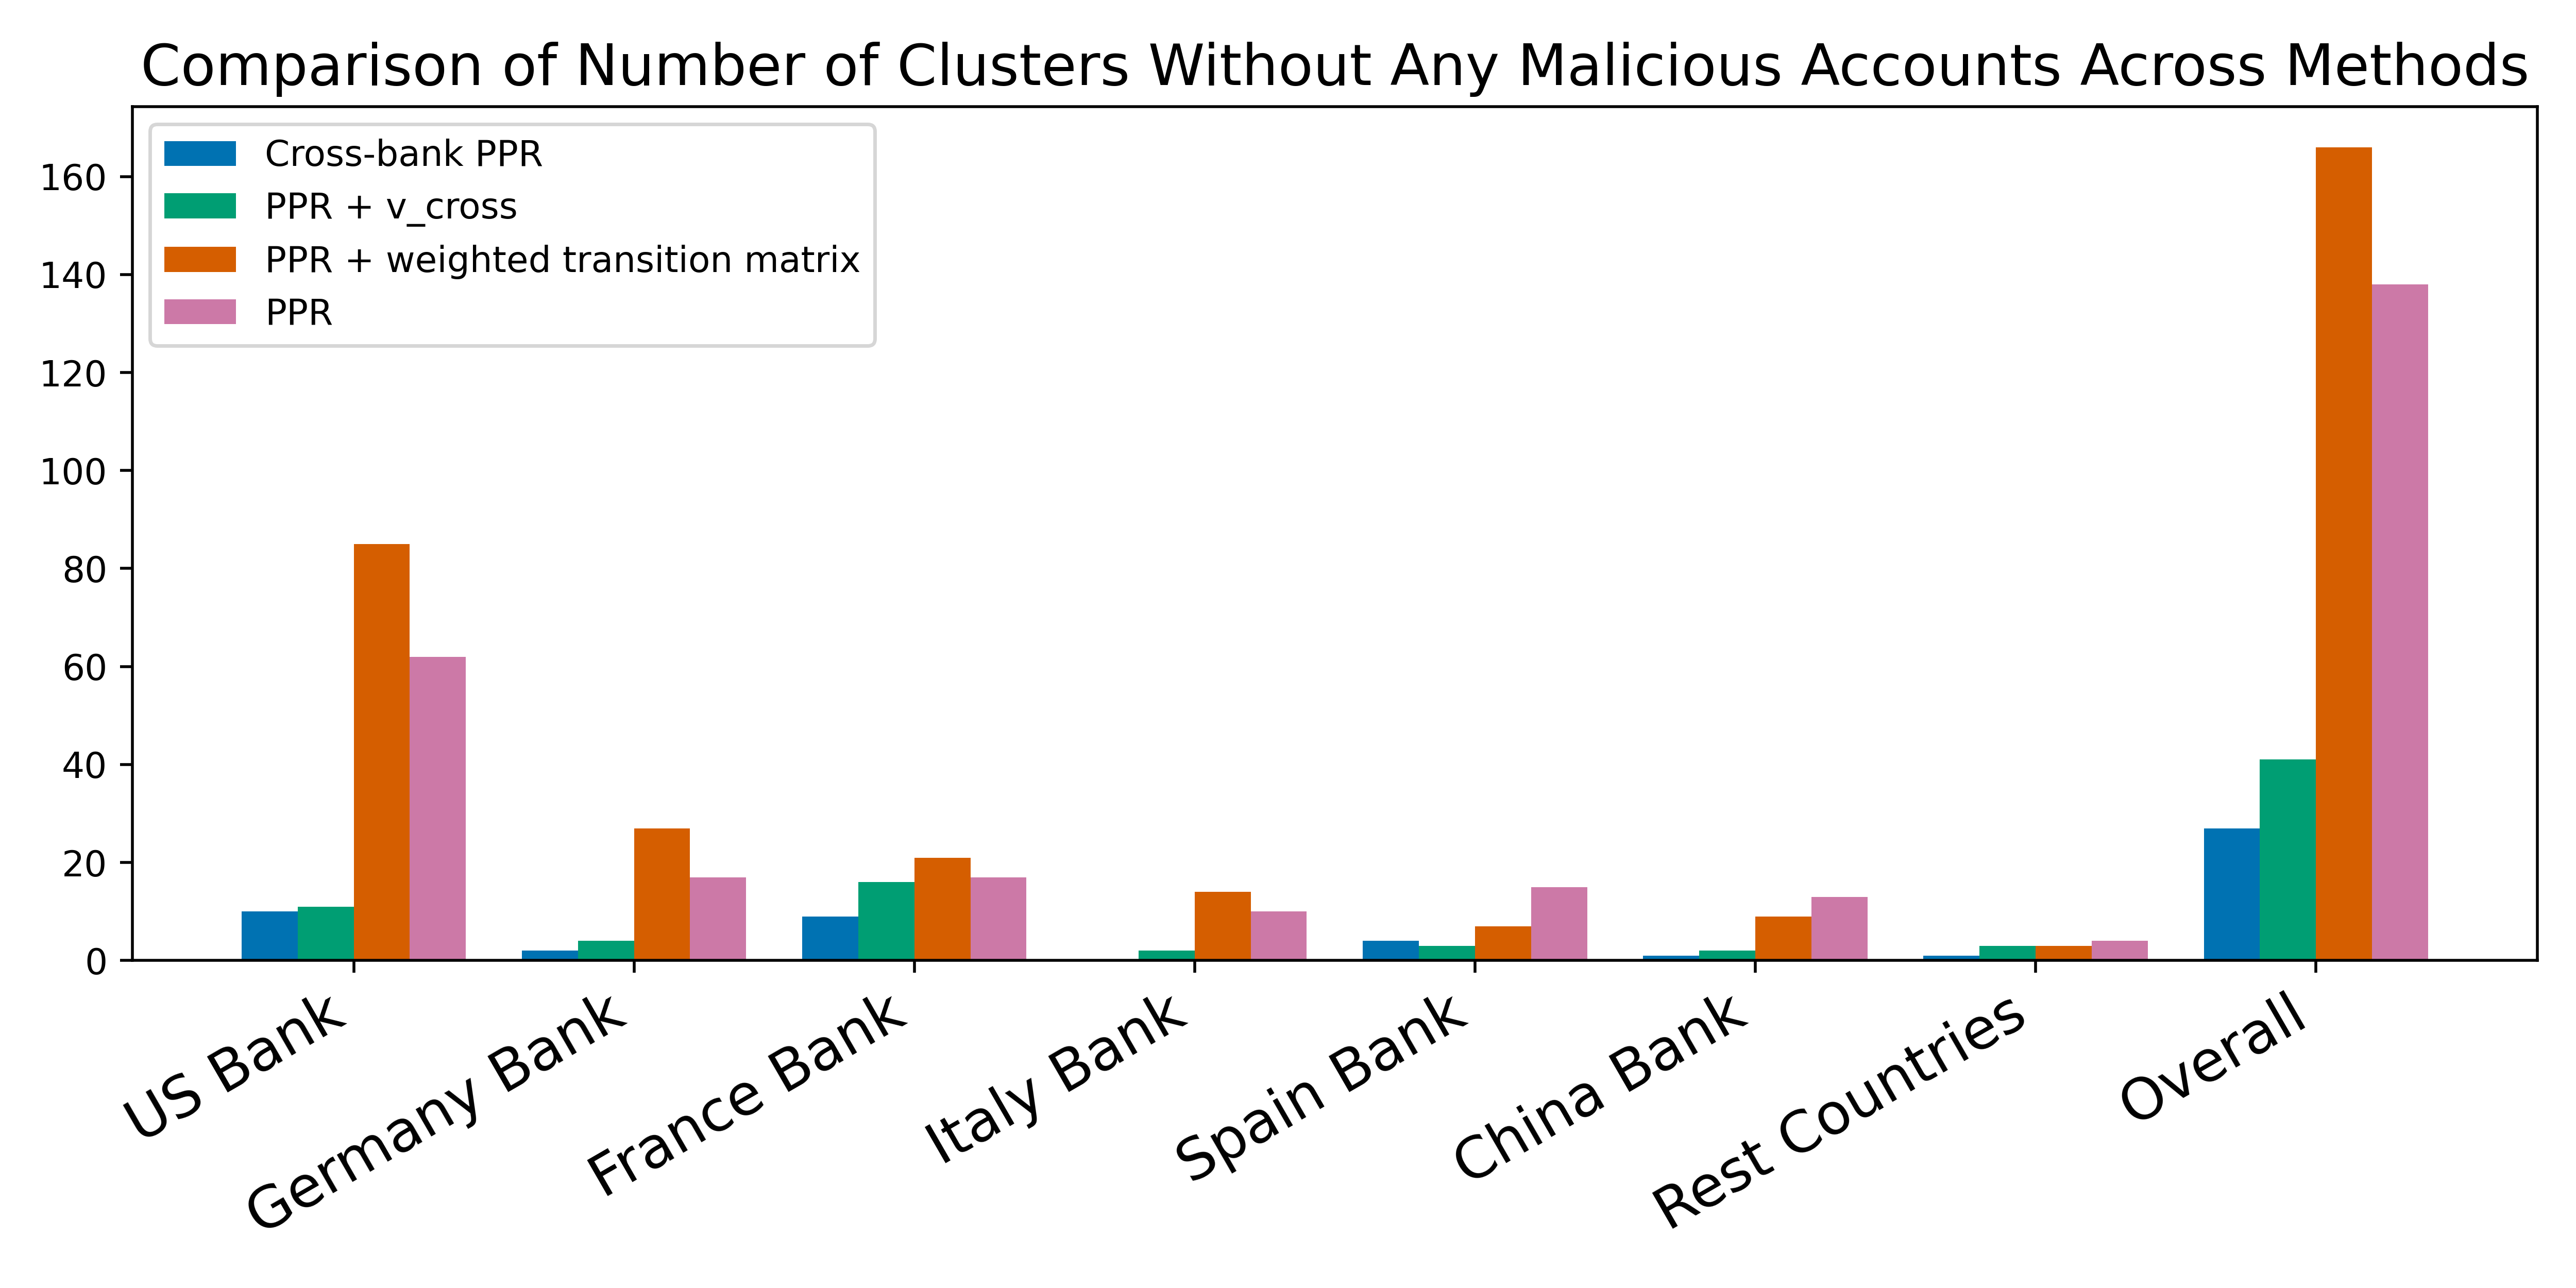
\includegraphics[width=\linewidth]{PPR_results/NoAnomalyCluster.png}
        \begin{center}
            \caption{Number of clusters containing no \\
            malicious accounts}
        \end{center}
    \end{subfigure}%
    \hfill
    \begin{subfigure}{0.5\linewidth}
        \centering
        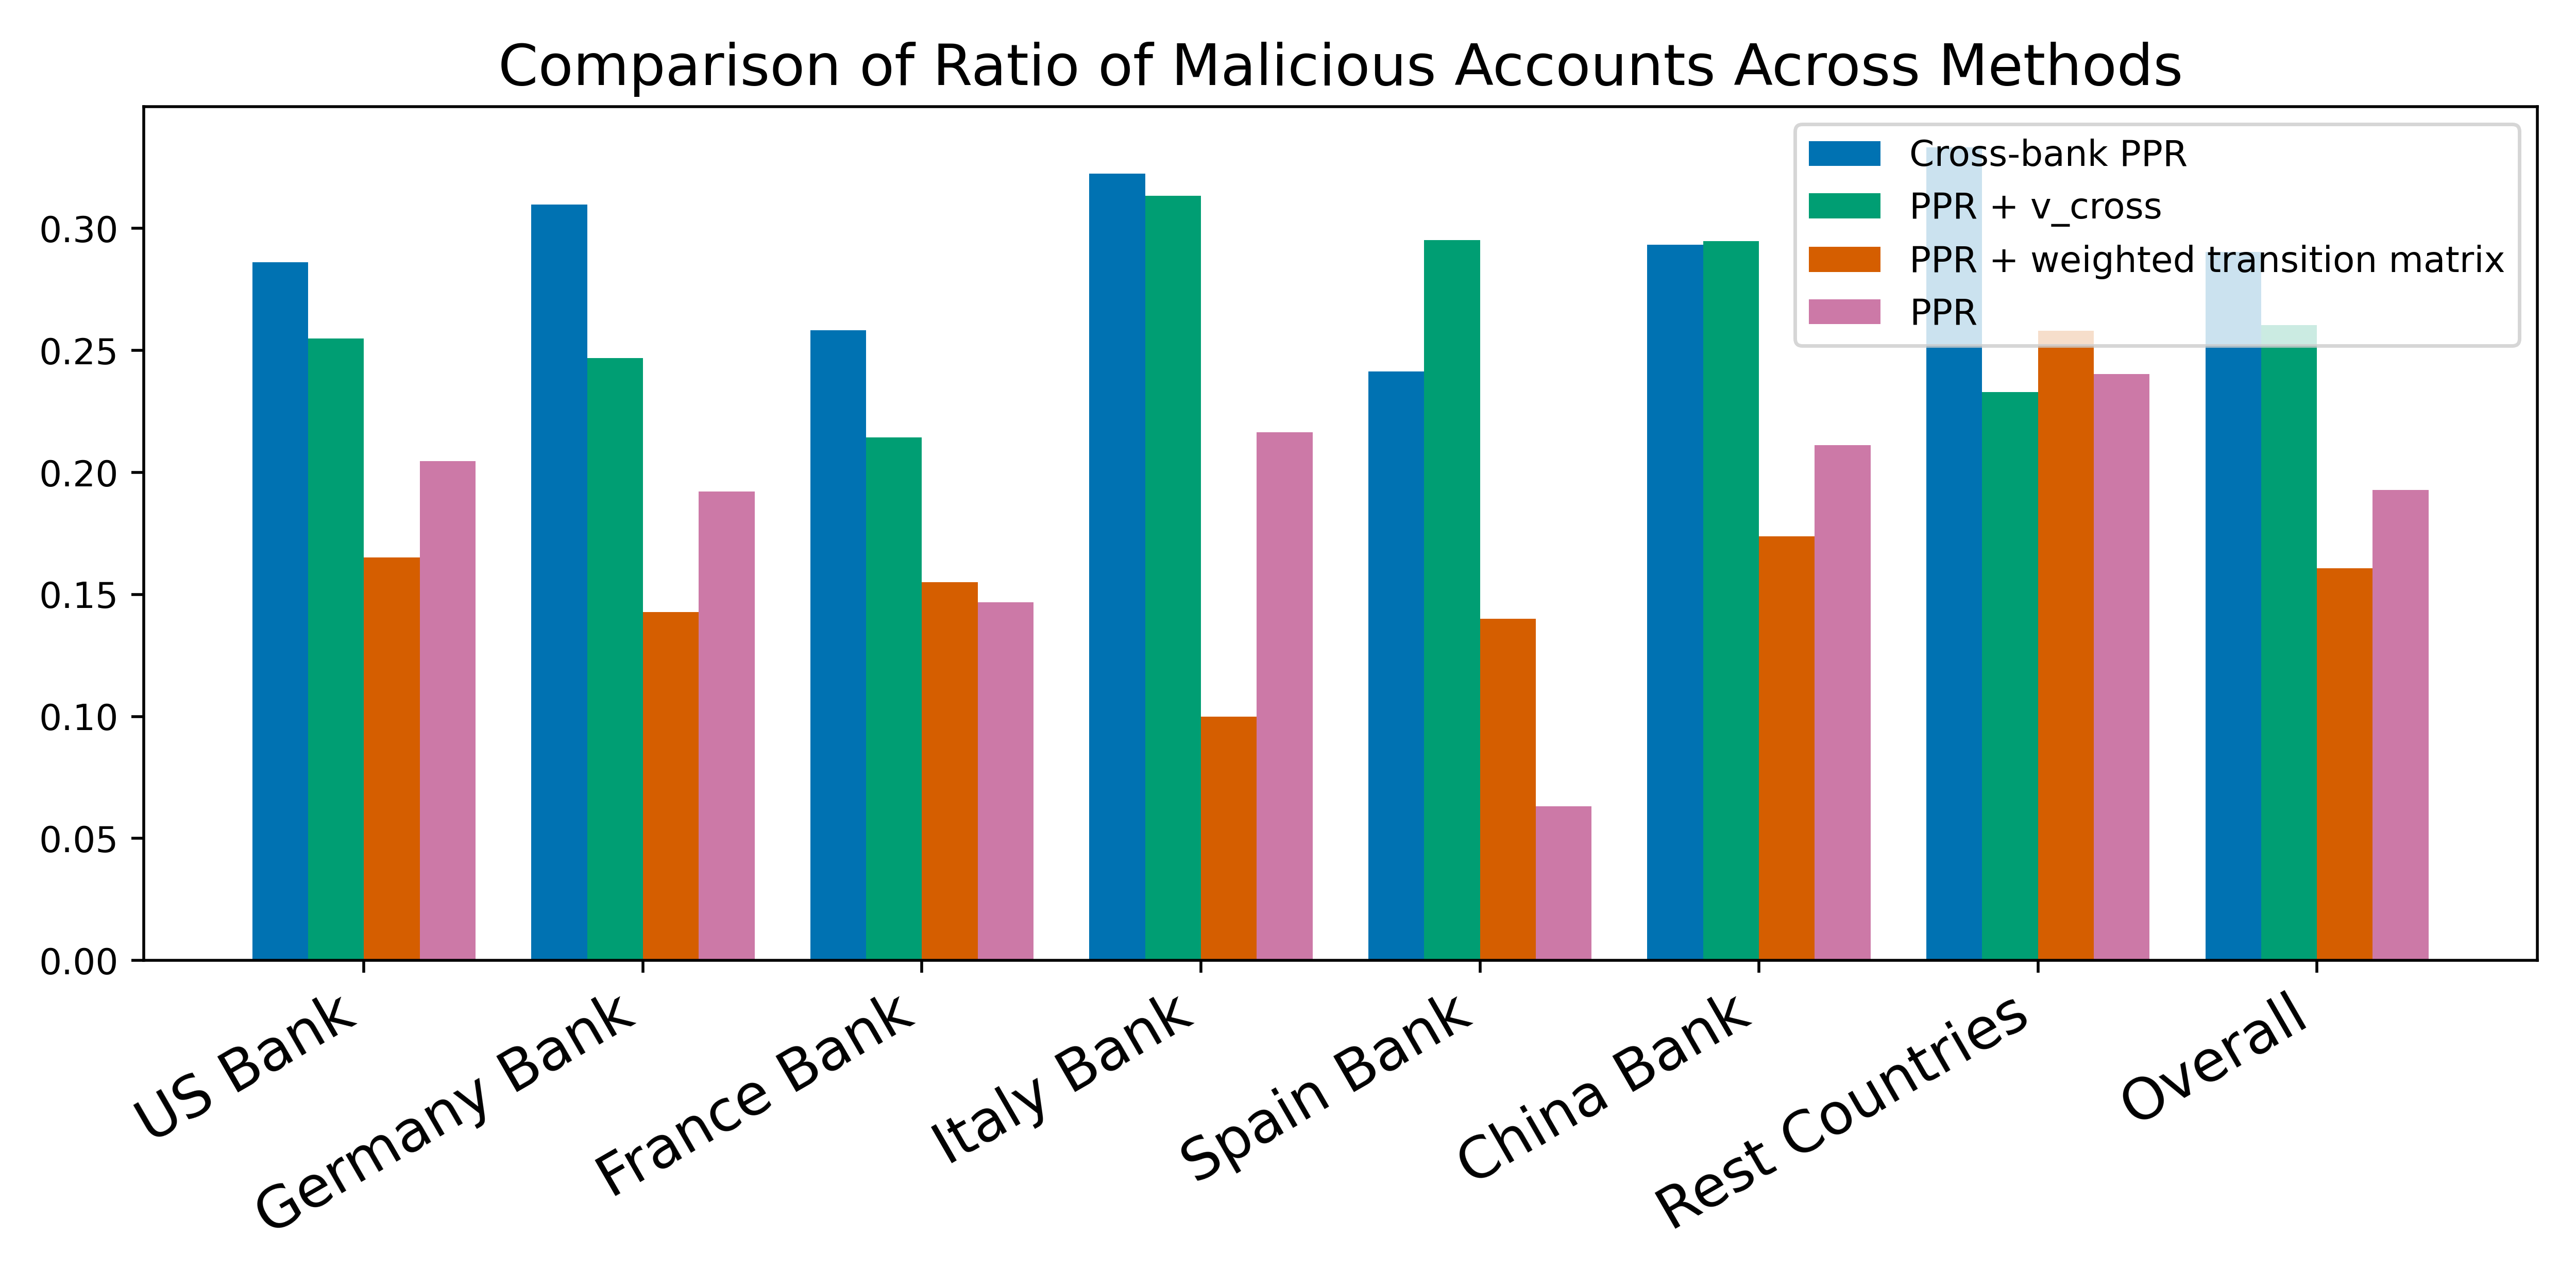
\includegraphics[width=\linewidth]{PPR_results/Anomaly_Ratio.png}
        \begin{center}
            \caption{Overall proportion of malicious \\
            accounts}
        \end{center}
    \end{subfigure}
    \vspace{0.5em} % small vertical space between rows
    
    \caption{Comparison between Cross-bank PPR and PPR}
    \label{fig:PPR_evaluation}
\end{figure}

\subsubsection{Effectiveness of Cross-bank PPR}
In this subsection, we examine the hypothesis that Cross-bank PPR improves malicious-account detection and reduces false positives, compared with PPR. To verify this hypothesis, we compare cross-bank PPR with vanilla PPR. Figure \ref{fig:PPR_evaluation} reports summary statistics for clusters generated by Cross-bank PPR, its two ablated variants, and standard PPR. The statistics include: the total number of accounts included across all clusters, the number of identified malicious accounts, the number of clusters containing no malicious accounts, and the overall proportion of malicious accounts (malicious accounts divided by total accounts).
Combining the results from Figures \ref{fig:PPR_evaluation} (a) and (b), we observe that Cross-bank PPR identifies fewer suspicious accounts overall than the other methods, yet it discovers substantially more true malicious accounts. This pattern indicates that Cross-bank PPR is simultaneously more conservative in flagging suspicious neighbors but more accurate in finding genuinely malicious ones. This cautiousness is further supported by Figure \ref{fig:PPR_evaluation} (c), which shows that Cross-bank PPR produces the fewest clusters with no malicious accounts, indicating fewer false positives and more targeted clustering. Finally, Figure \ref{fig:PPR_evaluation} (d) demonstrates that Cross-bank PPR achieves the highest malicious-account identification rate across most countries, as well as the highest overall performance.

Next, we evaluate the effectiveness of two key components (i.e., introducing the cross-bank component $v_{cross}$ and adding the edge prediction score $\hat{y}_{ij}$ into the transition matrix) of cross-bank PPR compared with vanilla PPR. When the cross-bank suspicious signal ($v_{cross}$) is incorporated into PPR, we improve the capability of this new variant (`PPR + v\_cross' in Figure \ref{fig:PPR_evaluation}) detecting malicious accounts and reduce the false positives, compared with PPR. This can be verified by the fewer suspicious accounts overall than PPR, more true malicious accounts included across all clusters, and less clusters with no malicious accounts, shown in \ref{fig:PPR_evaluation} (a), (b) and (c). Different from the effectiveness of cross-bank suspicious signal ($v_{cross}$), when we only incorporate the edge malicious score ($\hat{y}_{ij}$) to update the weighted transition matrix into PPR (denoted as `PPR + weighted transition matrix' in Figure \ref{fig:PPR_evaluation}), we immediately observe the performance drops across all four statistics in Figure \ref{fig:PPR_evaluation}. 
Notice that Theorem~\ref{thm:detectability} reveals a detectability condition for identifying a money-laundering group using Personalized PageRank (PPR) and whether the money-laundering group is well-separated heavily rely on the quality of the weighted transition matrix. Therefore, we conjecture that the edge malicious score by a single bank is not reliable and incorporating the unreliable score into the weighted transition matrix only leads to the worse results than PPR. Crucially, when $\hat{y}_{ij}$ is combined with $v_{cross}$ in Cross-bank PPR, its previously unreliable signal is corrected, yielding superior performance. This demonstrates that the two components are complementary and jointly critical for achieving high precision and effectiveness in malicious-account detection.

Together, these results highlight that both components ($v_{cross}$ and $\hat{y}_{ij}$) play a critical role in improving the precision and effectiveness of Cross-bank PPR in identifying malicious financial activity. Unlike standard PPR, Cross-bank PPR identifies fewer accounts overall but captures substantially more true malicious accounts, demonstrating higher precision in detecting risky entities. This cautious yet effective behavior is a key advantage in financial monitoring.

Identifying module and decision-making module play complementary roles: Cross-bank PPR produces structured, interpretable group signals under fragmentation, while the hierarchical decision model translates these signals into economically optimal interventions. Importantly, the decision layer remains robust even when group structures are partially observed, reflecting realistic cross-border compliance conditions. 
% While this section focuses on constructing interpretable group-level signals, their marginal economic value is quantified in the next section.

\subsubsection{Effectiveness of Label Propagation}
\label{effectivenss_label_propagation}
\begin{table}[t]
\centering
\caption{Detection performance with and without label propagation.}
\label{tab:label_propagation}
\resizebox{\linewidth}{!}{
\begin{tabular}{l|cccc|cccc}
\hline
 & \multicolumn{4}{c|}{\textbf{Without Label Propagation}} 
 & \multicolumn{4}{c}{\textbf{With Label Propagation}} \\
\hline
\textbf{Market} 
 & AUCROC & AUPRC & Type I & Type II 
 & AUCROC & AUPRC & Type I & Type II \\
\hline
United States        & 0.9819 & 0.6878 & 0.0459 & 0.0786 & 0.9820 & 0.6903 & 0.0534 & 0.0655 \\
Germany   & 0.9790 & 0.6007 & 0.0702 & 0.0455 & 0.9790 & 0.6025 & 0.0695 & 0.0478 \\
France    & 0.9788 & 0.5595 & 0.0686 & 0.0557 & 0.9788 & 0.5622 & 0.0706 & 0.0526 \\
Italy     & 0.9782 & 0.5867 & 0.0634 & 0.0755 & 0.9784 & 0.5991 & 0.0650 & 0.0645 \\
Spain     & 0.9802 & 0.5356 & 0.0603 & 0.0530 & 0.9802 & 0.5360 & 0.0651 & 0.0491 \\
China     & 0.9742 & 0.4949 & 0.0601 & 0.0504 & 0.9745 & 0.5091 & 0.0677 & 0.0358 \\
Rest Countries & 0.9861 & 0.8004 & 0.0398 & 0.0526 & 0.9862 & 0.8038 & 0.0410 & 0.0415 \\
\hline
\textbf{Overall} 
               & 0.9798 & 0.6094 & 0.0583 & 0.0588 
               & \textbf{0.9799} & \textbf{0.6147} & 0.0618 & \textbf{0.0510} \\
\hline
\end{tabular}
}
\end{table}



In this section, we validate the hypothesis that the discovered group-wise laundering patterns can be further exploited to improve detection performance through label propagation, as summarized in Table~\ref{tab:label_propagation}. Overall, incorporating propagated group-level signals consistently improves detection accuracy across all evaluated transaction subgraphs. In particular, we observe systematic gains in AUPRC for every bank-level subgraph, with especially notable improvements in more challenging settings such as China Bank and Italy Bank. These results indicate that label propagation is effective at recovering suspicious nodes and transactions that initially receive low confidence scores but are structurally connected to high-confidence laundering groups. Across all subgraphs, the AUCROC remains stable or slightly improves after label propagation, indicating that the refinement step does not degrade the model’s global discrimination ability. While we observe modest increases in Type I error rates for some graphs (e.g., US Bank and Spain Bank), these increases are accompanied by notable reductions in Type II errors in several cases, most prominently for China Bank and the aggregated Rest Countries graph. This trade-off reflects the intended behavior of label propagation: prioritizing recall of coordinated laundering activity by propagating malicious signals within densely connected groups, even at the cost of a small increase in false positives. These results confirm that group-wise laundering patterns captured by cross-bank PPR provide complementary information beyond edge-level predictions. By integrating this information through label propagation, the detection modu moves beyond isolated transaction analysis and leverages collective behavioral evidence, leading to more robust identification of coordinated money laundering activity across heterogeneous financial networks. We next evaluate the economic value of label propagation by incorporating it into the decision-making module to quantify its impact on prevented losses and resource allocation in the follow section.




\subsection{Empirical Results of Decision-Making Module}
\subsubsection{Economic Value of Hierarchical Decision-Making Module}
% \lc{To do list: 1. Regulatory Budget Constraint Experiment by imposing an intervention budget, such as Max 1\% of transactions frozen. -> What if regulators cap how many freezes you can issue? We can compare the Fixed threshold vs Hierarchical RL and report the prevented Loss under budget and missed laundering loss. This reframes your work as resource allocation under constraints—a classic MS theme. 2. Marginal value of cross-bank PPR experiment by comparing the economic value of hierarchical adaptive threshold with label-propagation vs without label-propagation. }
A central question for financial institutions is the economic value generated by a more sophisticated intervention mechanism. Specifically, how much financial loss can the proposed hierarchical decision-making module avert relative to traditional, fixed-threshold approaches? To address this, we estimate both the total financial loss attributable to money-laundering transactions and the prevented loss achieved when intervention policies are deployed by (i) a decision-making module with a fixed threshold and (ii) our hierarchical decision-making module. Table~\ref{tab:economic_values} summarizes these results in Panels A and B, respectively.

Our empirical analysis is conducted on the IBM Anti–Money Laundering (AML) dataset, which contains more than 1.4 million transaction records collected between September 1 and September 10, 2022. To emulate a realistic operational environment, we partition the data chronologically: the first 80\% of transactions (September 1–8) are sued for model training, while the remaining 20\% (September 8–10) are used exclusively for evaluation. Within the first part, we further split the data into equal halves for training and validation. We define  \textit{Threshold} as the threshold to freeze the suspicious transactions, \textit{Total Loss} as the aggregated dollar amount associated with successfully executed illicit transactions and \textit{Prevented Loss} as the amount that would have been blocked had the recommended intervention (i.e., transaction freezing) been deployed at the time of execution. We first train the federated graph-based detection modu (Section~\ref{sec:detection_model}) on the training data to produce transaction-level maliciousness scores across the training, validation and test sets. These scores in training set are then used to train the hierarchical decision-making module, which learns optimal thresholding policies for interventions. Hyperparameters are selected using the validation set. During evaluation, we also track Type I and Type II errors to capture the operational quality of intervention decisions. A missed freeze on a money-laundering transaction is counted as a false negative (Type II error), while an unnecessary freeze on a legitimate transaction is counted as a false positive (Type I error). These error metrics reflect the business risks of either failing to prevent financial crime or unnecessarily disrupting customer activity.


\begin{table}[htp]
\centering
\caption{Comparison of decision-making module with Fixed Threshold and Hierarchical decision-making module Performance Across Countries. The fixed threshold in Panel A is selected based on the overall threshold in Panel B for fair comparison.}
\resizebox{0.9\textwidth}{!}{
\begin{tabular}{lcccccc}
\hline
\multicolumn{7}{c}{\textbf{Panel A: Decision-making module with fixed threshold}} \\
\hline
\textbf{Market} & \textbf{Threshold} & \textbf{Total Loss} & \textbf{Prevented Loss} & \textbf{Prevented Loss Ratio} & \textbf{Type I Error} & \textbf{Type II Error} \\
\hline
United States   & 0.3974 & \$456.41 Million & \$252.43 Million & 0.5531 & 0.0178 & 0.4152 \\
Germany         & 0.3974 & \$357.24 Million & \$201.59 Million & 0.5643 & 0.0125 & 0.5830 \\
France          & 0.3974 & \$212.05 Million & \$110.13 Million & 0.5194 & 0.0119 & 0.5546 \\
Italy           & 0.3974 & \$223.72 Million & \$101.80 Million & 0.4550 & 0.0089 & 0.6141 \\
Spain           & 0.3974 & \$280.05 Million & \$57.51 Million  & 0.2053 & 0.0094 & 0.5933 \\
China           & 0.3974 & \$292.43 Million & \$147.15 Million & 0.5032 & 0.0116 & 0.6140 \\
Rest Countries  & 0.3974 & \$118.45 Million & \$88.10 Million  & 0.7438 & 0.0069 & 0.4610 \\
\textbf{Overall} & 0.3974 & \$1940.35 Million & \$958.70 Million & 0.4941 & 0.0113 & 0.5479 \\
\hline
\end{tabular}}
\resizebox{0.9\textwidth}{!}{
\begin{tabular}{lcccccc}
\multicolumn{7}{c}{\textbf{Panel B: Hierarchical Decision-Making Module (without Label Propagation)}} \\
\hline
\textbf{Market} & \textbf{Threshold} & \textbf{Total Loss} & \textbf{Prevented Loss} & \textbf{Prevented Loss Ratio} & \textbf{Type I Error} & \textbf{Type II Error} \\
\hline
United States & 0.3163 & \$456.41 Million & \$455.29 Million & 0.9975 & 0.1029 & 0.0554 \\
Germany & 0.4195 & \$357.24 Million & \$343.75 Million & 0.9622 & 0.0348 & 0.3138 \\
France & 0.5226 & \$212.05 Million & \$24.32 Million & 0.1147 & 0.0083 & 0.6753 \\
Italy & 0.3163 & \$223.72 Million & \$223.60 Million & 0.9995 & 0.1023 & 0.0403 \\
Spain & 0.4711 & \$280.05 Million & \$80.30 Million & 0.2868 & 0.0150 & 0.5075 \\
China & 0.3679 & \$292.43 Million & \$292.01 Million & 0.9985 & 0.0847 & 0.1462 \\
Rest Countries & 0.3679 & \$118.45 Million & \$118.36 Million & 0.9993 & 0.0654 & 0.0487 \\
\textbf{Overall} & 0.3974 & \$1940.35 Million & \$1537.64 Million & 0.7925 & 0.0591 & 0.2553 \\
\hline
\end{tabular}}
\resizebox{0.9\textwidth}{!}{
\begin{tabular}{lcccccc}
\multicolumn{7}{c}{\textbf{Panel C: Hierarchical Decision-Making Module with Label Propagation}} \\
\hline
\textbf{Market} & \textbf{Threshold} & \textbf{Total Loss} & \textbf{Prevented Loss} & \textbf{Prevented Loss Ratio} & \textbf{Type I Error} & \textbf{Type II Error} \\
\hline
United States & 0.3679 & \$456.41M & \$442.96M & 0.9705 & 0.0650 & 0.0964 \\
Germany & 0.3163 & \$357.24M & \$356.92M & 0.9991 & 0.0775 & 0.0789 \\
France & 0.4711 & \$212.05M & \$141.62M & 0.6678 & 0.0189 & 0.3190 \\
Italy & 0.6258 & \$223.72M & \$50.46M & 0.2255 & 0.0011 & 0.7490 \\
Spain & 0.4195 & \$280.05M & \$227.58M & 0.8126 & 0.0327 & 0.2276 \\
China & 0.3163 & \$292.43M & \$280.09M & 0.9578 & 0.0797 & 0.0731 \\
Rest Countries & 0.4195 & \$118.45M & \$118.08M & 0.9968 & 0.0140 & 0.1721 \\
\textbf{Overall} & 0.4195 & \$1,940.35M & \$1,617.71M & 0.8337 & 0.0413 & 0.2452 \\
\hline
\end{tabular}}
\label{tab:economic_values}
\end{table}

When using a fixed threshold of 0.3974 (the threshold is selected based on the overall threshold in Panel B), the model prevents 49.41\% of total financial loss. This low prevented-loss ratio reveals that the fixed-threshold mechanism fails to translate predictive signals into effective business actions. The high Type II error rate of 54.79\% further underscores this issue that the model does not freeze the vast majority of illicit transactions, allowing substantial losses to occur. From a risk management perspective, such performance indicates that a one-size-fits-all thresholding policy is ill-suited for complex, heterogeneous transaction environments. Differently, Panel B provides strong evidence that the hierarchical decision-making module substantially enhances intervention effectiveness. The model prevents 79.25\% of the potential financial loss, which is over 60\% improvement over the fixed-threshold baseline. The significant reduction in Type II error from 54.79\% to 25.53\% demonstrates that the model more reliably identifies and disrupts illicit flows, improving both operational accuracy and economic efficiency. Interestingly, we also observe that the learned intervention thresholds vary across bank branches in different countries (ranging from 0.3163 to 0.5226), suggesting that optimal risk tolerance levels are context-dependent. This finding has practical implications for multinational financial institutions that uniform thresholding may mask local transaction behaviors, whereas adaptive, hierarchical policies can better align with regional risk patterns. Importantly, the combination of learned thresholds and low Type II error indicates that a lower maliciousness score, particularly one near the threshold, does not necessarily imply normal behavior. Rather, these scores must be interpreted in combination with the model’s learned hierarchical decision logic. These findings demonstrate that the model’s ability to tailor intervention thresholds to regional patterns offers a scalable way to harmonize global compliance requirements with local risk dynamics beyond improving accuracy. For financial institutions facing rising regulatory scrutiny and increasingly sophisticated money-laundering schemes, such models can deliver both economic value and operational resilience.

In Section~\ref{effectivenss_label_propagation}, we have demonstrated the effectiveness of label propagation of incorporating the results of cross-bank PPR. One key question arises: \textit{What is the economic value of label propagation based on the structural signals discovered through cross-bank PPR?} To answer this, we evaluate the financial impact of integrating label propagation into the hierarchical decision-making framework. Table~\ref{tab:economic_values} Panel B and C compares the performance of the hierarchical decision-making module with and without label propagation across countries. Overall, integrating label propagation increases the total prevented loss from \$1,537.64M to \$1,617.71M and improves the prevented loss ratio from 0.7925 to 0.8337, demonstrating a substantial enhancement in loss mitigation. Type I errors decrease from 0.0591 to 0.0413, indicating fewer false alarms, while Type II errors slightly decrease overall (0.2553 → 0.2452), reflecting a minor improvement in detection of unprevented losses. At the country level, the effects vary: for example, the United States sees a reduction in Type I error (0.1029 → 0.0650) but a small increase in Type II error (0.0554 → 0.0964), whereas Germany achieves near-complete loss prevention (prevented loss ratio 0.9622 → 0.9991) with balanced error rates. Smaller markets, including Rest Countries, maintain consistently high intervention efficiency under both models. These results indicate that incorporating label propagation into the hierarchical decision-making framework enhances global mitigation of financial losses, improves overall robustness against false positives, and maintains effective detection across diverse market structures.


\subsubsection{Economic Value of Hierarchical Decision-Making Module Under Regulatory Budget Constraint}
\begin{table}[htbp]
\centering
\caption{Comparison of Fixed Threshold and Label Propagation under a Fixed Budget Constraint. Thresholds are not reported, with a maximum intervention budget of 1\% of transactions.}
\resizebox{0.9\textwidth}{!}{
\begin{tabular}{lccccc}
\hline
\multicolumn{6}{c}{\textbf{Panel A: Decision-Making Module with Fixed Threshold Under Fixed Budget Constraint}} \\
\hline
\textbf{Market} & \textbf{Total Loss} & \textbf{Prevented Loss} & \textbf{Prevented Loss Ratio} & \textbf{Type I Error} & \textbf{Type II Error} \\
\hline
United States & \$456.41M & \$23.996M & 0.0526 & 0.0017 & 0.7982 \\
Germany & \$357.24M & \$55.766M & 0.1561 & 0.0013 & 0.8057 \\
France & \$212.05M & \$23.983M & 0.1131 & 0.0015 & 0.7902 \\
Italy & \$223.72M & \$50.583M & 0.2261 & 0.0016 & 0.8087 \\
Spain & \$280.05M & \$1.289M & 0.0046 & 0.0019 & 0.8284 \\
China & \$292.43M & \$19.927M & 0.0681 & 0.0016 & 0.8538 \\
Rest Countries & \$118.45M & \$35.556M & 0.3002 & 0.0003 & 0.7987 \\
\textbf{Overall} & \$1,940.35M & \$211.10M & 0.1088 & 0.0014 & 0.8120 \\
\hline
\end{tabular}}
\resizebox{0.9\textwidth}{!}{
\begin{tabular}{lccccc}
\multicolumn{6}{c}{\textbf{Panel B: Hierarchical Decision-Making Module with Label Propagation Under Fixed Budget Constraint}} \\
\hline
\textbf{Market} & \textbf{Total Loss} & \textbf{Prevented Loss} & \textbf{Prevented Loss Ratio} & \textbf{Type I Error} & \textbf{Type II Error} \\
\hline
United States & \$456.41M & \$82.393M & 0.1805 & 0.0056 & 0.5911 \\
Germany & \$357.24M & \$92.672M & 0.2594 & 0.0091 & 0.5749 \\
France & \$212.05M & \$0.142M & 0.0007 & 0.0508 & 0.1092 \\
Italy & \$223.72M & \$56.804M & 0.2539 & 0.0069 & 0.6644 \\
Spain & \$280.05M & \$37.419M & 0.1336 & 0.0031 & 0.7015 \\
China & \$292.43M & \$11.531M & 0.0394 & 0.0045 & 0.6813 \\
Rest Countries & \$118.45M & \$0.377M & 0.0032 & 0.0140 & 0.1721 \\
\textbf{Overall} & \$1,940.35M & \$281.34M & 0.1450 & 0.0134 & 0.4992 \\
\hline
\end{tabular}}
\label{tab:fixed_budget}
\end{table}

In practice, regulatory authorities face strict constraints on how many interventions they can deploy. For instance, regulators may be allowed to freeze only a small fraction of transactions—say, 0.5\%—to avoid disrupting normal operations and to comply with operational or legal limits. Under such a budget constraint, the key challenge is not just detecting suspicious activity, but allocating limited intervention resources effectively across diverse markets and transaction networks. This reframes anti-money-laundering efforts as a classical resource allocation problem: given a fixed budget of interventions, how can regulators maximize prevented losses while minimizing missed laundering activity?

Table~\ref{tab:fixed_budget} addresses this question by comparing a fixed-threshold strategy with label propagation under the same intervention budget. With a fixed threshold, the system behaves very conservatively: overall, only \$211.10 Million financial losses are prevented with 0.1088 of Prevented loss ratio, and Type II errors are extremely high (0.8120), meaning most laundering activity are not intervened. 0.0014 of Type I errors, however, are almost negligible, reflecting that the limited intervention budget is spent on the normal transactions. By contrast, the hierarchical decision-making module prioritizes interventions more strategically. Specifically, total prevented loss increases to \$281.34 Million with 0.1450 of prevented loss ratio, while Type II errors drop significantly to 0.4992, showing a much higher capture of laundering activity under the same budget. This improvement comes with a modest increase in Type I errors from 0.14\% to 1.34\%, reflecting a slight increase in false positives that is acceptable given the large gain in prevented losses. At the country/market level, the impact is even more illustrative. High-risk and high-volume markets, such as the US and Germany, see substantial improvements in prevented losses, while smaller markets maintain effective coverage without overspending the limited budget. These results demonstrate that hierarchical decision-making module effectively leverages structural connections among suspicious nodes to guide interventions under resource constraints, translating enhanced detection performance into real economic value. In other words, by propagating group-level laundering signals, the system learns where to “spend” its limited freezes most effectively, making regulatory intervention more efficient and impactful.



% \subsubsection{Marginal Value of Label Propagation}
% \begin{table}[htbp]
% \centering
% \caption{Comparison of Hierarchical Decision-Making Model With and Without Label Propagation Across Countries. Thresholds are selected per market for optimal performance.}
% \resizebox{0.9\textwidth}{!}{
% \begin{tabular}{lcccccc}
% \hline
% \multicolumn{7}{c}{\textbf{Panel A: Hierarchical Decision-Making Module}} \\
% \hline
% \textbf{Market} & \textbf{Threshold} & \textbf{Total Loss} & \textbf{Prevented Loss} & \textbf{Prevented Loss Ratio} & \textbf{Type I Error} & \textbf{Type II Error } \\
% \hline
% United States & 0.3163 & \$456.41M & \$455.29M & 0.9975 & 0.1029 & 0.0554 \\
% Germany & 0.4195 & \$357.24M & \$343.75M & 0.9622 & 0.0348 & 0.3138 \\
% France & 0.5226 & \$212.05M & \$24.32M & 0.1147 & 0.0083 & 0.6753 \\
% Italy & 0.3163 & \$223.72M & \$223.60M & 0.9995 & 0.1023 & 0.0403 \\
% Spain & 0.4711 & \$280.05M & \$80.30M & 0.2868 & 0.0150 & 0.5075 \\
% China & 0.3679 & \$292.43M & \$292.01M & 0.9985 & 0.0847 & 0.1462 \\
% Rest Countries & 0.3679 & \$118.45M & \$118.36M & 0.9993 & 0.0654 & 0.0487 \\
% \textbf{Overall} & 0.3974 & \$1,940.35M & \$1,537.64M & 0.7925 & 0.0591 & 0.2553 \\
% \hline
% \end{tabular}}
% \resizebox{0.9\textwidth}{!}{
% \begin{tabular}{lcccccc}
% \multicolumn{7}{c}{\textbf{Panel B: Hierarchical Decision-Making Module with Label Propagation}} \\
% \hline
% \textbf{Market} & \textbf{Threshold} & \textbf{Total Loss} & \textbf{Prevented Loss} & \textbf{Prevented Loss Ratio} & \textbf{Type I Error} & \textbf{Type II Error} \\
% \hline
% United States & 0.3679 & \$456.41M & \$442.96M & 0.9705 & 0.0650 & 0.0964 \\
% Germany & 0.3163 & \$357.24M & \$356.92M & 0.9991 & 0.0775 & 0.0789 \\
% France & 0.4711 & \$212.05M & \$141.62M & 0.6678 & 0.0189 & 0.3190 \\
% Italy & 0.6258 & \$223.72M & \$50.46M & 0.2255 & 0.0011 & 0.7490 \\
% Spain & 0.4195 & \$280.05M & \$227.58M & 0.8126 & 0.0327 & 0.2276 \\
% China & 0.3163 & \$292.43M & \$280.09M & 0.9578 & 0.0797 & 0.0731 \\
% Rest Countries & 0.4195 & \$118.45M & \$118.08M & 0.9968 & 0.0140 & 0.1721 \\
% \textbf{Overall} & 0.4195 & \$1,940.35M & \$1,617.71M & 0.8337 & 0.0413 & 0.2452 \\
% \hline
% \end{tabular}}
% \label{tab:hierarchical_labelprop}
% \end{table}


